%\documentclass[review]{elsarticle}
%\documentclass[preprint]{elsarticle}
%\documentclass[1p]{elsarticle}
%\documentclass[3p]{elsarticle}
%\documentclass[5p]{elsarticle}
\documentclass[final,5p,times,twocolumn]{elsarticle}
%\documentclass[final,5p,twocolumn]{elsarticle}
\usepackage[russian,english]{babel}
\usepackage[utf8]{inputenc} % Включаем поддержку UTF8
%\usepackage[T2A]{fontenc}


\usepackage{lineno}
\usepackage{graphicx}
\usepackage{xcolor}
\usepackage[pdftex, backref, colorlinks]{hyperref}

\modulolinenumbers[5]
%\journal{Journal of \LaTeX\ Templates}
%\journal{Journal}
\journal{}

%%%%%%%%%%%%%%%%%%%%%%%
%% Elsevier bibliography styles
%%%%%%%%%%%%%%%%%%%%%%%
%% To change the style, put a % in front of the second line of the current style and
%% remove the % from the second line of the style you would like to use.
%%%%%%%%%%%%%%%%%%%%%%%

%% Numbered
%\bibliographystyle{model1-num-names}

%% Numbered without titles
%\bibliographystyle{model1a-num-names}

%% Harvard
%\bibliographystyle{model2-names.bst}\biboptions{authoryear}

%% Vancouver numbered
%\usepackage{numcompress}\bibliographystyle{model3-num-names}

%% Vancouver name/year
%\usepackage{numcompress}\bibliographystyle{model4-names}\biboptions{authoryear}

%% APA style
%\bibliographystyle{model5-names}\biboptions{authoryear}

%% AMA style
%\usepackage{numcompress}\bibliographystyle{model6-num-names}

%% `Elsevier LaTeX' style
\bibliographystyle{elsarticle-num}
%%%%%%%%%%%%%%%%%%%%%%%
%\hyphenpenalty=10000

\begin{document}
\begin{frontmatter}
\title{Observation of reflected EAS Cherenkov light with the SPHERE-2 detector}
\author[address1]{R.A.~Antonov}
\author[address1]{E.A.~Bonvech\corref{correspondingauthor1}}
\cortext[correspondingauthor1]{Corresponding author}
\ead{bonvech@yandex.ru}
\author[address1]{D.V.~Chernov}
\author[address1]{T.A.~Dzhatdoev}
\author[address2]{V.I.~Galkin}
\author[address2,address1]{D.A.~Podgrudkov}
\author[address1]{T.M.~Roganova}
\author[address2]{I.A.~Vaiman}
\address[address1]{Federal State Budget Educational Institution of Higher Education, M.V. Lomonosov Moscow State University, Skobeltsyn Institute of Nuclear Physics (SINP MSU), 1(2), Leninskie gory, GSP-1, 119991 Moscow, Russia}
\address[address2]{Federal State Budget Educational Institution of Higher Education, M.V. Lomonosov Moscow State University, Department of Physics, 1(2), Leninskie gory, GSP-1, 119991 Moscow, Russia}

\begin{abstract}
The paper presents some results of the data processing of the observations of reflected EAS Cherenkov light in the SPHERE experiment. The compact detector SPHERE-2 was lifted to 400--900~m altitude above snow covered surface of Lake Baikal during 2008--2013 seasons and Vavilov-Cherenkov radiation of extensive air showers generated by super high energy cosmic ray particles in the Earth atmosphere was registered. SPHERE is the first experiment in which the reflected EAS Cherenkov light was recorded and events with the Cherenkov signal were identified.
\end{abstract}
\begin{keyword}
primary cosmic rays\sep extensive air showers\sep Vavilov--Cherenkov radiation\sep ballon
\MSC[2010] 00-01\sep  99-00
\end{keyword}
\end{frontmatter}
\linenumbers

%\tableofcontents


\begin{figure*}[tb]
\begin{minipage}[t]{0.47\textwidth}
\centering
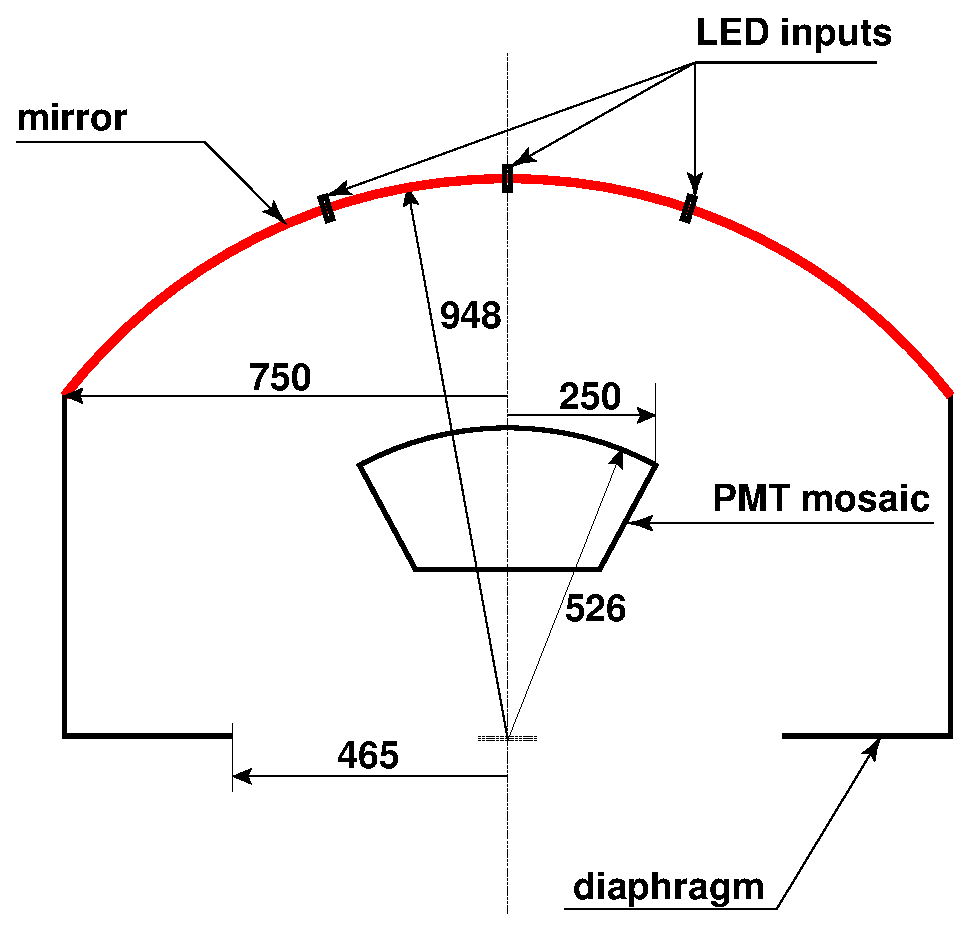
\includegraphics[width=17pc]{figs/optics_side}\hspace{2pc}%
\caption{Optical scheme of the \mbox{SPHERE-2} detector.}
\label{fig:optics}
\end{minipage}
\hfill
\begin{minipage}[t]{0.47\textwidth}
\centering
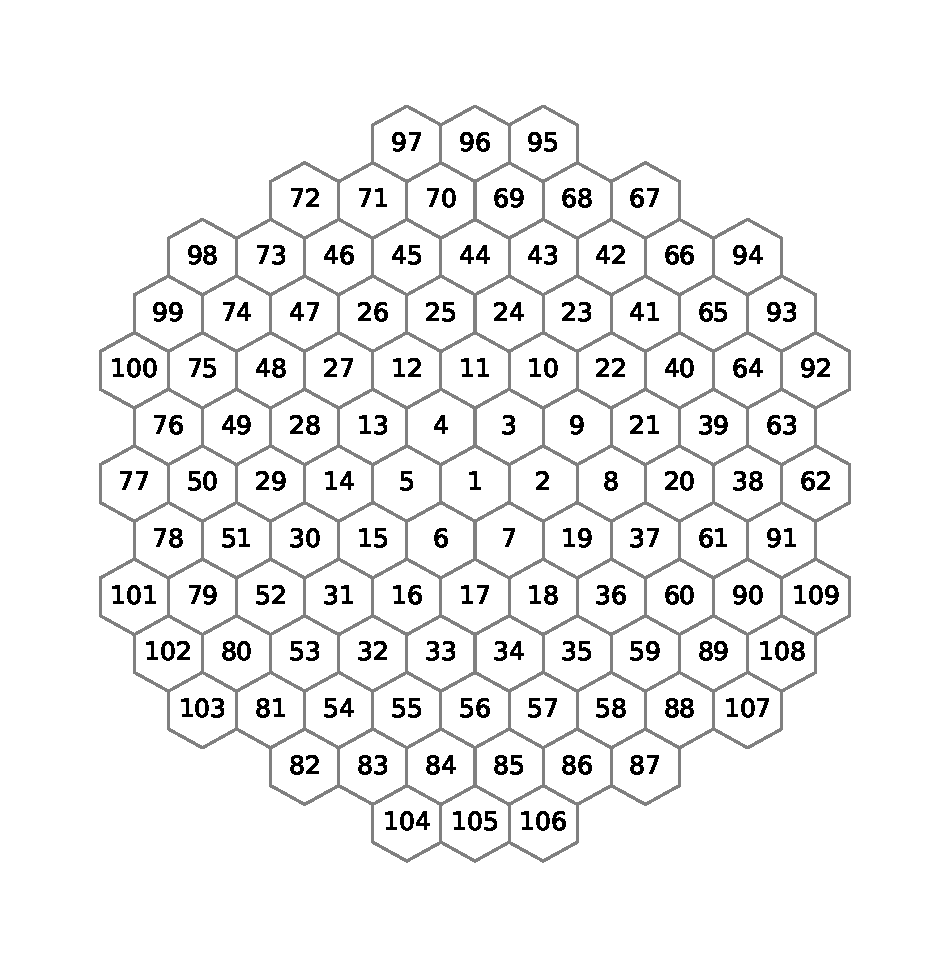
\includegraphics[width=19pc]{figs/retina.eps}%
\vspace{-1.0pc}
\caption{The PMT retina of the SPHERE-2 detector with PMTs numbers indicated.}
\label{fig:retina}
\end{minipage}
\end{figure*}

\section{Introduction}

Extensive air showers (EAS) --- cascades of particles in the Earth atmosphere --- allow to study cosmic rays (CR) in a wide energy region $E$ from 1~PeV to 100~EeV ($10^{15}$--$10^{20}$ eV), recording fluxes as small as one particle per 1000 km$^{2}$ per year~\cite{abu12,aab15,abb08,iva09}. Besides hadrons, leptons and high-energy $\gamma$-rays, EAS also produce optical photons by means of Vavilov-Cherenkov radiation (hereafter simply `Cherenkov light', CL)~\cite{bla47} and air fluorescence~\cite{chu62, suga62}. EAS CL in the atmosphere has sharp angular profile peaked in the direction of the primary nucleus while fluorescent light (FL) is isotropic. CL and FL photons are the most numerous component of EAS, their number is several orders of magnitude greater than the number of charged particles and high energy $\gamma$-rays combined. These optical radiations may travel many kilometers in the atmosphere without strong absorption and thus they represent a good remote probe of EAS. 

Modern EAS arrays such as the Telescope Array (TA) detector and the Pierre Auger Observatory (PAO) are ground-based structures spread over hundreds~\cite{abu12} or thousands~\cite{aab15} square kilometers. Significant efforts are needed in order to install sensitive elements of such vast arrays and to keep them power-supplied and time-synchronized. Therefore, it is very tempting to use a compact device to observe EAS. Fluorescent light of EAS can be observed by Earth-based detectors~\cite{abu12,aab15,abb08,fly75} due to its isotropic angular distribution. Direct EAS Cherenkov light in the atmosphere, however, typically has a very sharp directional pattern and could not be observed by detectors more than 1 km far from the shower axis. On the other hand, CL reflected from natural surfaces such as snow could indeed be recorded due to diffuse reflection pattern of such surfaces~\cite{chu74, ant99, ant15a, ant19}. EAS FL also may be observed by a space-based~\cite{lin81, adam15a} or balloon-based~\cite{adam15c} detector.

Search for fluorescent tracks of EAS appeared to be a very hard task beyond the capabilities of present-day experiments and analyses. Indeed, no clear events of such kind were reported yet~\cite{abd18, tus18}. In this paper we report on observation of reflected CL events with the SPHERE-2 detector~\cite{ant15a}. This is the first detailed study of such kind. In total, we found more than one thousand EAS events. We note that our approach to analyses and our technique for search of EAS events could be helpful for other experiments such as JEM-EUSO balloon or JEM-EUSO. The paper is organized as follows. In Sect.~\ref{sect:detector} we describe the SPHERE-2 detector. (...). 

{\Russian
Здесь еще нужно поработать.
}

Finally, we summarize in Conclusions.



\section{The SPHERE-2 detector \label{sect:detector}}

The SPHERE is a cosmic ray experiment based on the registration of Vavilov-Cherenkov radiation generated by extensive air showers (EAS) in the atmosphere and reflected from the snow covered ground surface. The experiment is aimed at accurate registration and reconstruction of every event allowing the event-by-event approach to the EAS primary particle identification and primary spectra study. The present paper is dedicated to the SPHERE experiment stage performed with the compact detector SPHERE-2 in Baikal Lake region during 2009--2013 winter seasons. The previous stages of the SPHERE experiment are decribed in~\cite{ant15a}.

The \mbox{SPHERE-2} detector is a compact optical device to measure the EAS Cherenkov light from the balloon elevated to altitudes up to 3~km above the Earth snow covered surface. Special tethered balloon BAPA developed and created by Russian Augur agency for this experiment was used.

\subsection{Optics system}

The \mbox{SPHERE-2} detector optics consists of a 1.5~m diameter spherical mirror with a 109 photomultiplier tube (PMT) retina as on the Fig.~\ref{fig:optics}. 

The PMT retina is located near the mirror focal surface and records the Cherenkov light reflected from the snow surface below the detector. PMTs are arranged in the hexagonal structure on the spherical surface as shown on Fig.~\ref{fig:retina}. The central PMT of the retina is the Hamamatsu-R3686 photomultiplier and the others are the FEU-84-3 PMTs. The fields of view of PMTs are fixed in angular terms. The exact shape of the area that a single PMT observes depends on the PMT's position in the retina and the detector orientation.

\subsection{Electronics}

The electronics part includes a data acquisition system (DAQ), trigger system, calibration system etc. The DAQ contains a 10-bit flash analog-to-digital converters (FADC) with 40~MHz sampling frequency and provided 12.5~ns discretization using two \mbox{FADCs} per one optical channel. DAQ worked in a continuous mode first forking the signal from each PMT to trigger system and to a 6~$\mu$s delay line. The details on the \mbox{SPHERE-2} apparatus construction and DAQ system operation see in~\cite{ant15a}. 


\subsection{Trigger system}

The trigger system (TS) of the SPHERE-2 detector produces an `event' signal when the trigger condition is satisfied. The trigger condition was: 1~${\mu}$s time window -- so called `local' trigger $LN$ or in any $M$ PMTs -- `global' trigger $GM$. The number of channels to exceed the threshold level was varied from flight to flight to decrease the energy threshold, but the most of the data was obtained under trigger conditions `$L3$ OR $G5$' then one of two trigger conditions have to be satisfied. The posterior analysis shows that some events was recorded under trigger $L2$ although the condition $L3$ was set.


\subsection{Data acquisition} 

When the TS produced an `event' signal the DAQ started recording 12.8~$\mu$s of signal from the delay line including capturing $\sim 6~\mu$s of the signal prior to the trigger signal and formed an `event' dataframe. One detector `event' dataframe contains a 12.8~$\mu$s record of the PMT DAQ signal data from measuring channels with 12.5~ns discretization, in total 1020 10-bit signal values per every of 109 PMT channels. If the signal value exceeded the 10-bit number the 11$^{th}$ bit of the recorded signal value number was set to 1 to indicate the overflowing of the FADC counter and to 0 otherwise. A highest 12$^{th}$ bit of signal value number is set to 1 if the PMT signal exceeds the trigger level. In addition to PMT data the following event information is stored: GPS  coordinates, altitude, UTC time, local time, trigger time, angles of detector inclination, magnetometer data, every PMT average anode currents. One `event' frame information takes 220 kBytes.

All the data is saved to a binary file on the detector onboard computer hard drive. From primary binary files the work files were created during frames preprocessing. Preprocessing included baselines estimation and substraction, time drift detection and correction, for detail see~\ref{sect:preprocessing}.


\begin{table}[b]
\centering
\caption{The annual statistics of the SPHERE experiment on Baikal Lake}
\label{tab:statistics}
\vspace{1pc}
\begin{tabular}{|c||c|r|c|r|r|}
\hline
run  & flights & PMT    & time, & triggers \\ 
year &         & number & hours & detected \\ 
\hline \hline
\multicolumn{5}{|c|}{test runs} \\
\hline
2008 & 1 &  20 &  1 &     1 \\ 
2009 & 5 &  20 &  1 &     1 \\ 
\hline
\multicolumn{5}{|c|}{experiment runs} \\
\hline
2010 & 6 &  96 & 30 &  1343 \\
2011 & 4 &  96 & 30 & 20571 \\
2012 & 5 & 109 & 31 &  7716 \\
2013 & 5 & 109 & 33 &  3813 \\
\hline
\end{tabular}
\end{table}


\subsection{Calibration}

The PMT sensitivity depends on the temperature, background light, power supply and etc. The online calibration system was used to correctly account for PMT gain factors.

Each trigger `event' frame is paired in 6 $\mu$s by a follow-up `calibration event' that was saved in the same format of the data. The `calibration event' is caused by the illumination of the PMT retina by LEDs from the mirror surface level (see Fig.~\ref{fig:optics}) according to the calibration algorithm. Each LED produces individual flash with known light distribution over the PMT mosaic. 

The `calibration' frame is used to apply calibration and nonlinearity correction to each PMT channel in the trigger event it follows. The procedure for obtaining calibration and linearity corrections data is described in detail in the dedicated paper~\cite{ant16}. 

\begin{figure}[tb]
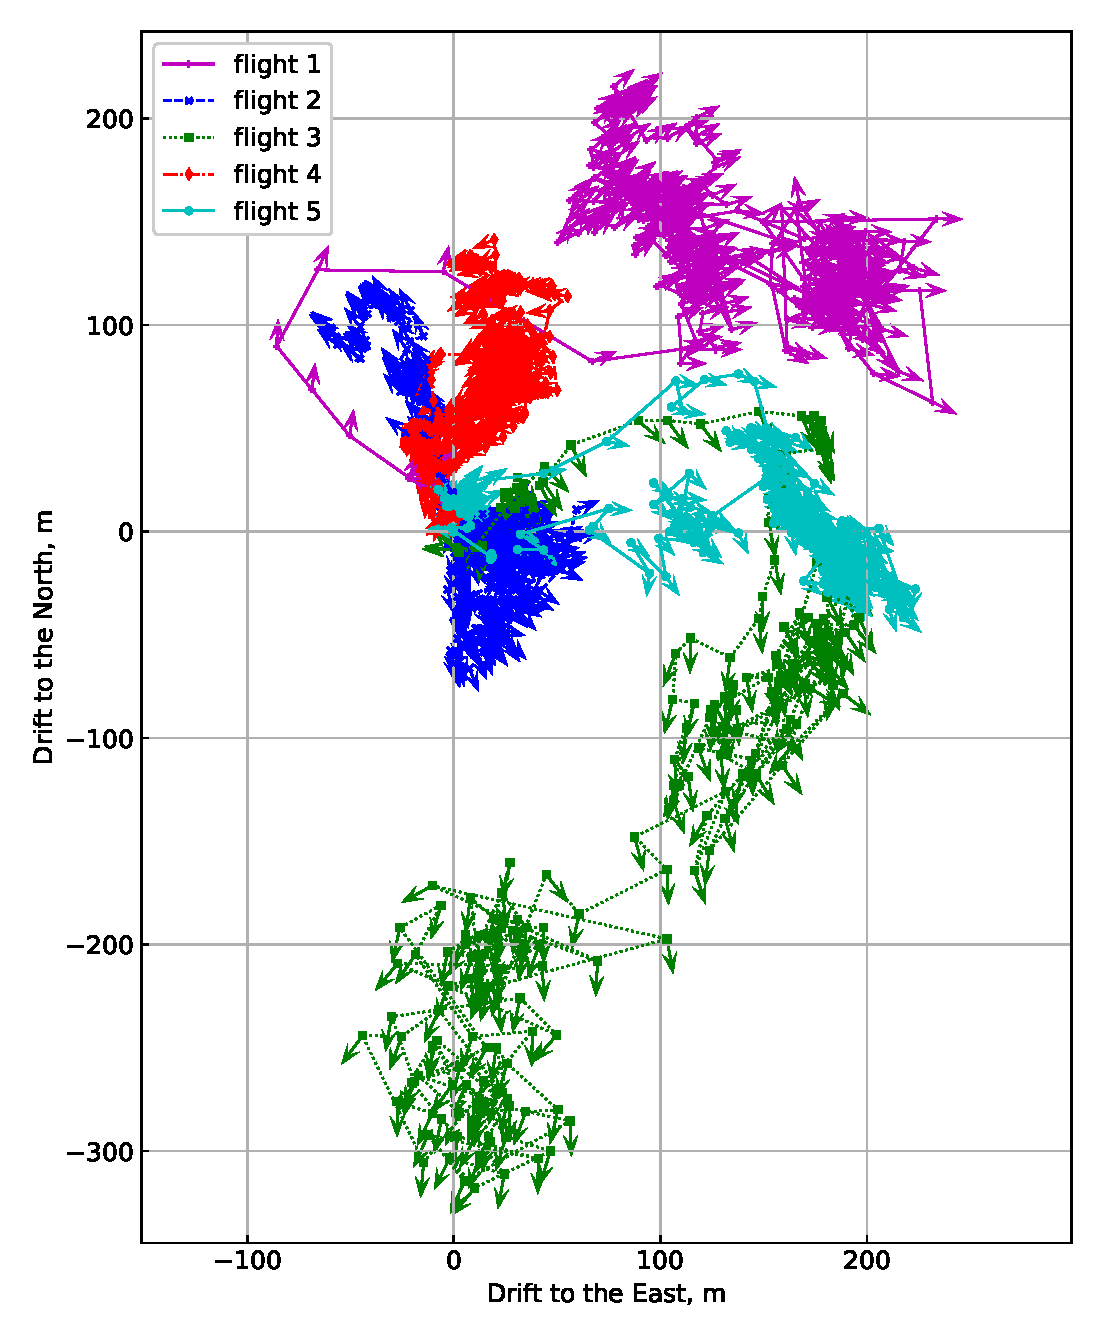
\includegraphics[width=0.49\textwidth]{figs/GPS+quiver.eps}\hspace{2pc}%
\caption{The SPHERE-2 detector drift during 2013 flight. The arrows indicate the detector magnetometer orientation. The start point is located at zero coordinates.}
\label{fig:gps_compass}
\end{figure}


\subsection{Detector orientation control system}

The detector axis at the rest state is oriented vertically and detector observes the snow covered lake surface just under the detector. During the measurements, the detector hanging under the balloon, swung and rotated freely. The detector inclination is an important factor for the shower parameters reconstruction as it determined the overall geometry of the experiment. To control the position and rotation of the detector an inclinometer and a magnetometer compass are installed on the PMT retina control board. 

The magnetometer compass measures the angle of the detector's orientation relative to the Earth's magnetic field with 0.1~degree precision.

%%%%%%%%%%%%%%
\begin{figure*}[tb]
    \begin{minipage}{0.48\textwidth}
    \centering
    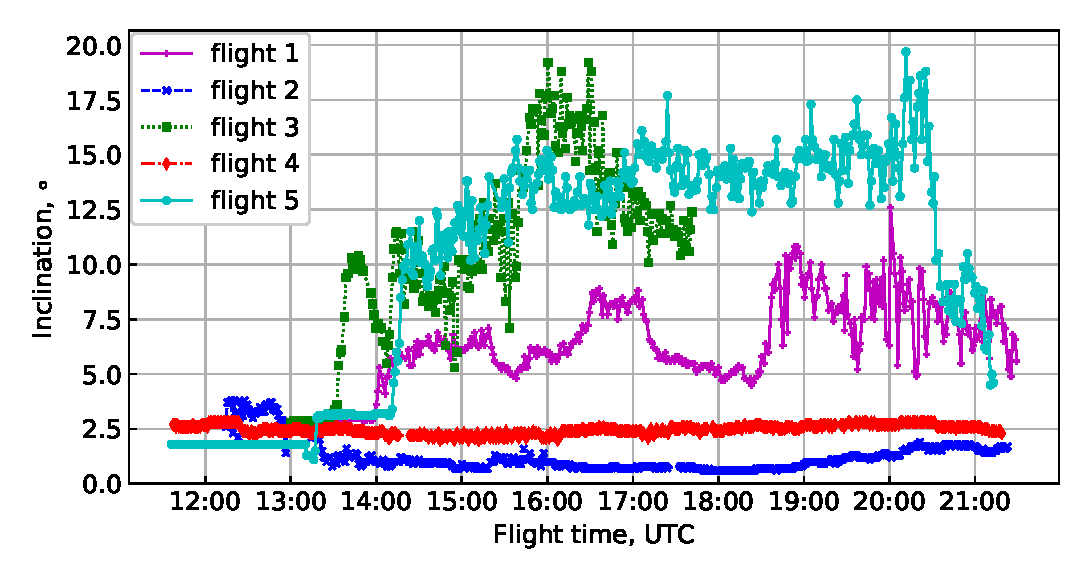
\includegraphics[width=\textwidth]{figs/ClinTh.eps}
    \caption{The detector inclination during 2013 experiment run according to the inclinometer data.}
    \label{fig:inclination} 
    \end{minipage}
    \hfill
    \begin{minipage}{0.48\textwidth}
    \centering
    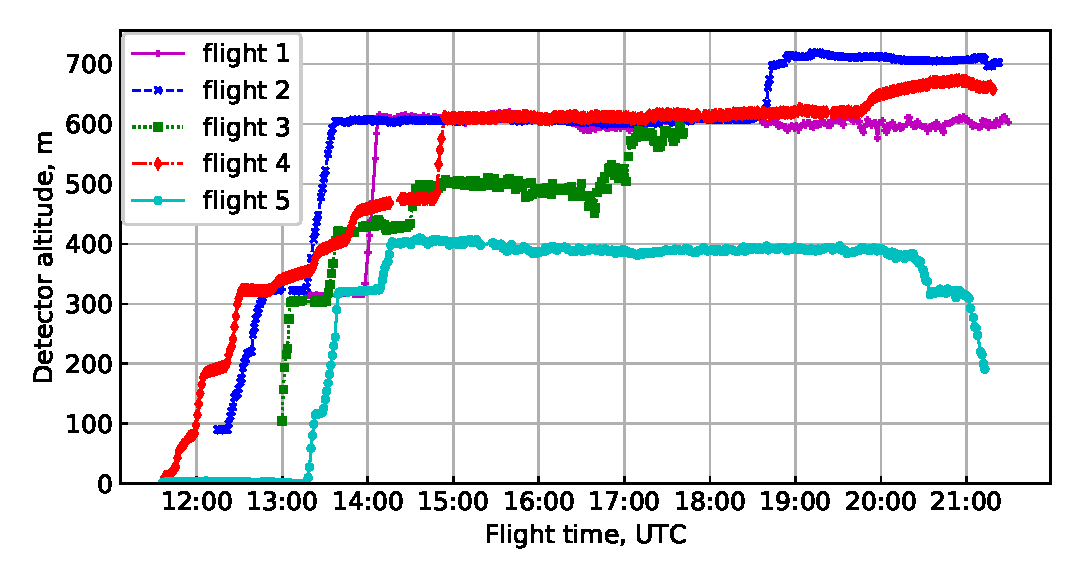
\includegraphics[width=\textwidth]{figs/height.eps}
    \caption{The altitude of the SPHERE-2 detector carried by the BAPA tethered balloon during 2013 experiment run according to the GPS module data.}
    \label{fig:height}
    \end{minipage}

  \vspace{1.5pc}

    \begin{minipage}{0.48\textwidth}
    \centering
    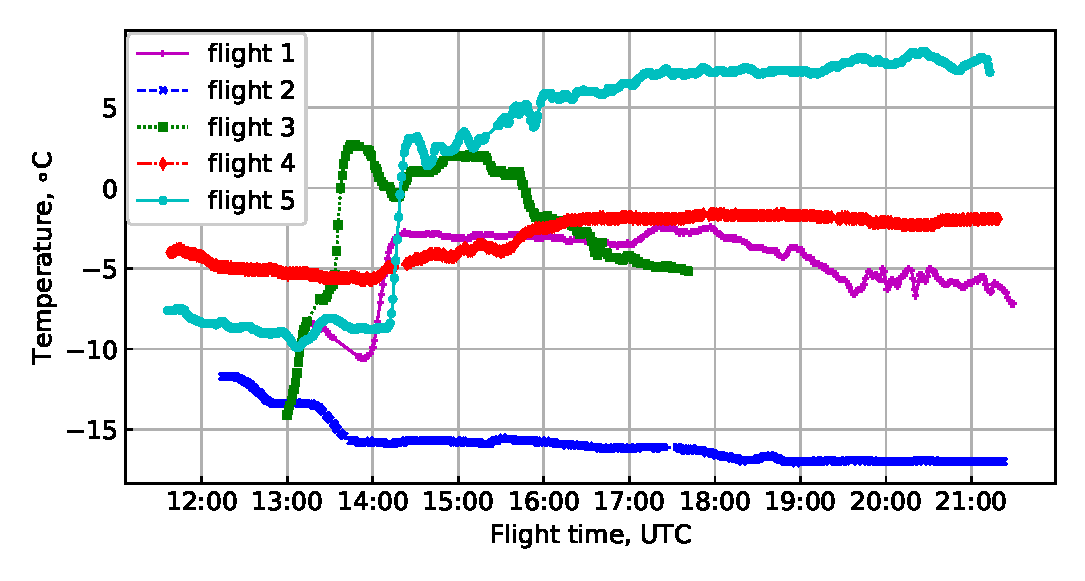
\includegraphics[width=\textwidth]{figs/T1.eps}
    \caption{The air temperature during 2013 run according to the barometer sensor data.}
    \label{fig:temperature}
    \end{minipage}
    \hfill
    \begin{minipage}{0.48\textwidth}
    \centering
    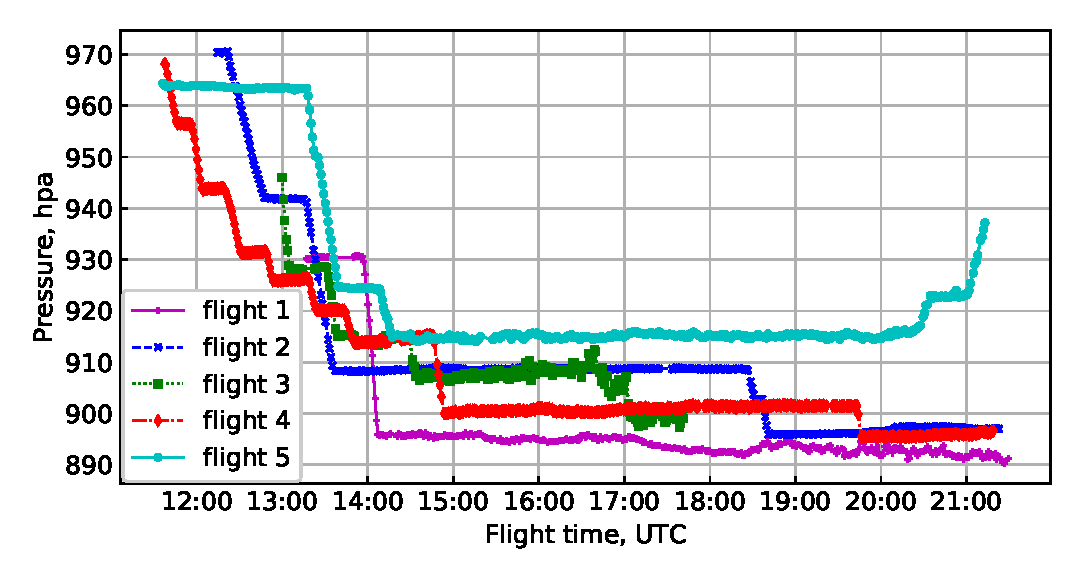
\includegraphics[width=\textwidth]{figs/P_hpa0.eps}
    \caption{The pressure during 2013 flights according to the barometer sensor data.}
    \label{fig:pressure}
    \end{minipage}
\end{figure*}
%%%%%%%%%%%%%%

The inclinometer measures two angles between it's internal orthogonal axes and the plane orthogonal to the gravity vector. The orientation of inclinometer axes respectively to detector retina axes was determined in the laboratory. After careful preparations the mosaic was set horizontally with precision better than $0.1^\circ$ and the zero level of the inclinometer was measured. All detector inclination angles were calculated considering recovered zero level.

The type of inclinometer used allows fast angles measurements with low power consumption, but, contrary to the gyroscopic ones, it is affected by acceleration. As we will see in sec~\ref{sect:telemetrydata} during detector flights there were no recorded strong wind gusts and the balloon position was stable. So we assumed that  registered by inclinometer angles were unaffected by swinging.

The GPS sensor Garmin 16xHVS, located on the control unit was used to measure coordinates and elevation above sea level.

\subsection{Telemetry monitoring\label{sect:telemetry}}

During every experimental flight a lot of information about the detector status and the environmental parameters is recorded. The different telemetry data is received and checked every second, every minute and every 10 minutes. 

Every second the detector position and orientation was recorded. The GPS data of altitude, latitude and longitude, universal global time UTC, the angles of detector inclination by the inclinometer sensor, magnetometer compass data and the control block inner temperature was monitored. The additional GPS and barometer were deployed on the Baikal Lake ice surface level.

Every minute the PMT and the power status was monitored. Anode currents of all photomultipliers, the PMT retina temperature and the temperature of the photomultipliers high voltage power source as well as the voltage of the batteries and of constant voltage sources were recorded. Barometer sensors were polled every minute also.

Every ten minutes the PMT supply voltage, voltage at the first and tenth dynodes, temperature were checked for each photomultiplier. The measuring channel counting rates and voltage on the FADC boards with the measuring channels were also recorded.



\section{Experimental data \label{sect:data}}

The SPHERE experiment was carried out on the Baikal Lake, Russia during winters 2008-2013. The Baikal lake ice thickness reaches 40-60 cm in February. The balloon launch pad was deployed on the frozen Baikal lake ice surface 800~m far from the shore in the point with coordinates near 51$^\circ$47'48.923''N, 104$^\circ$23'19.187"E. 
%51.796923~N, 104.388663~E http://www.google.com/maps?q=51.796923,+104.388663
The balloon attracted the attention of a large number of Baikal tourists. 

The \mbox{SPHERE-2} detector was lifted by the tethered balloon BAPA to altitudes up to 900~m above snow surface. The annual statistics of the experiment is given by the Table~\ref{tab:statistics}. The first two years were test ones. The detector configuration was improved from year to year. Thus the number of PMTs was increased from 96 to 109, the signal time sampling was changed in 2012 from 25 ns to 12.5~ns.

Unless otherwise specified, all illustrations in the paper are given for the \mbox{SPHERE-2} data of the winter 2013 run. All plots were made with Python Matplotlib plotting library.


\subsection{Weather and snow}

Measurements were carried out during clear moonless cloudless nights with low wind. The measurements were started 1.5 hour after sunset or immediately after moonset and were finished before moonrise or 1.5 hour before sunrise. If the wind condition had become unsuitable for the flight the balloon with detector was landed at once as it was in the third flight in 2013. The typical night air temperature on the lake surface was near -15~$^\circ$C. According to~\href{https://rp5.ru/}{'Raspisaniye Pogodi'} data archive of the nearest weather stations with numbers 30818 and 30710 the horizontal visibility was at least 10 km, and the height of the base of the lowest clouds was 2500~m and more or no clouds were present. The Milky Way was clearly visible all the nights.

Our experiment was carried out when the Baikal surface was covered with freshly fallen snow. The snow reflection properties were controlled by using a device sensitive to light intensity in the optical band (“luxmeter”). The influence of the snow state on its reflecting properties has been discussed in detail in our article on the simulation of the SPHERE-2 detector~\cite{ant19}. 


\subsection{Detector orientation and telemetry data\label{sect:telemetrydata}}

The \mbox{SPHERE-2} detector position and wind conditions near the detector are clear from the Fig.~\ref{fig:gps_compass} and Fig.~\ref{fig:inclination}. The Fig.~\ref{fig:gps_compass} demonstrates every minute \mbox{SPHERE-2} detector coordinates according to GPS sensor during flights of 2013 winter run. The start point is located at zero coordinates. The detector orientation measured by magnetometer is indicated by arrows. Figure~\ref{fig:gps_compass} demonstrates that wind was quite constant and the balloon position was rather stable. The balloon position was affected by the wind. But the detector orientation was stable in the wind flow and it did not rotate around its axis randomly during all the experiment.  

Under the influence of wind the SPHERE-2 detector was deflected by a small angle from the vertical axis. For example, as one can see on the Fig.~\ref{fig:inclination} in 2013 run during second and fourth flights the~\mbox{SPHERE-2} detector was suspended almost vertically, while in the others it was tilted by the wind but this declination was steady and varied slowly over time. The maximum inclination angle of the detector was about twenty degrees from vertical axis. The inclination effect was taken into account at the stage of EAS parameters reconstruction.

Fig.~\ref{fig:height} shows the detector altitude above lake ice surface according to the GPS module data. The surrounding air temperature and pressure are presented on the Fig.~\ref{fig:temperature} and Fig.~\ref{fig:pressure} respectively according to the data of the onboard pressure sensor.


\begin{figure}[tb]
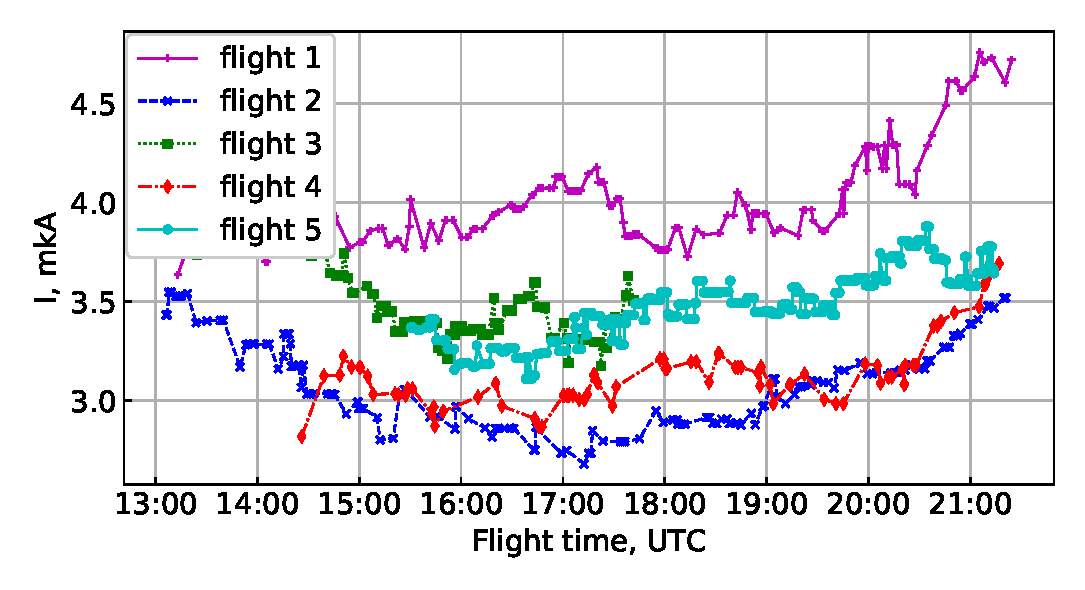
\includegraphics[width=0.48\textwidth]{figs/cur2013_PMT1.eps}
\caption{The central PMT current.}
\label{fig:current}
\end{figure}

\begin{figure}[t]
    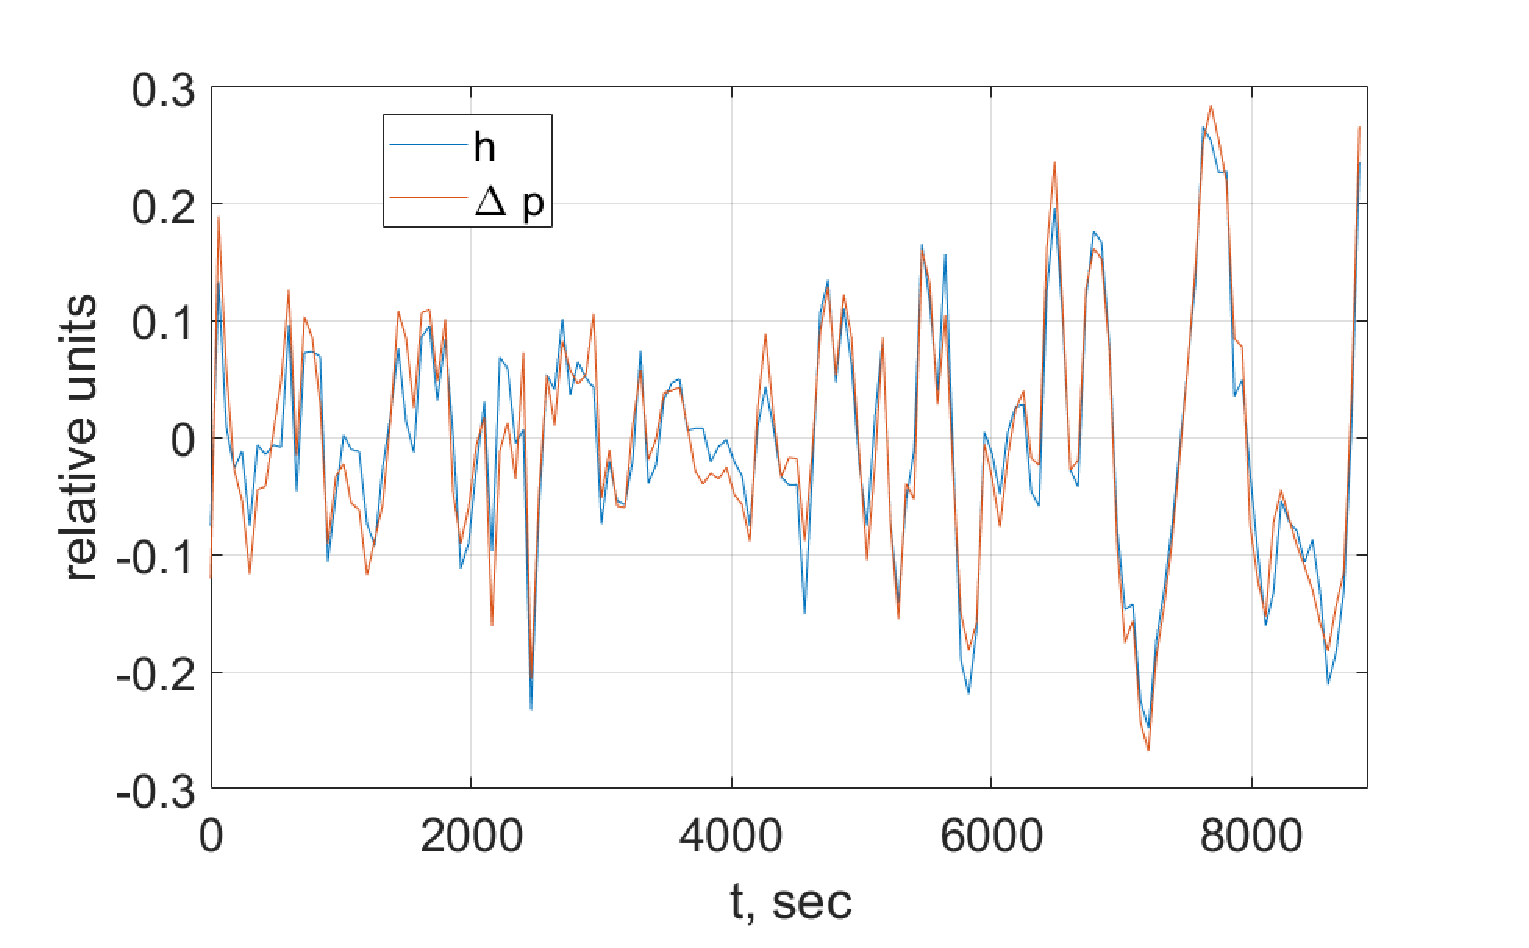
\includegraphics[width=0.48\textwidth]{figs/good_corr.eps}
    \caption{Balloon altitude is generally stable. Flight 3-2013 data.}
    \label{fig:dp-h-good}
    \vspace{1pc}

    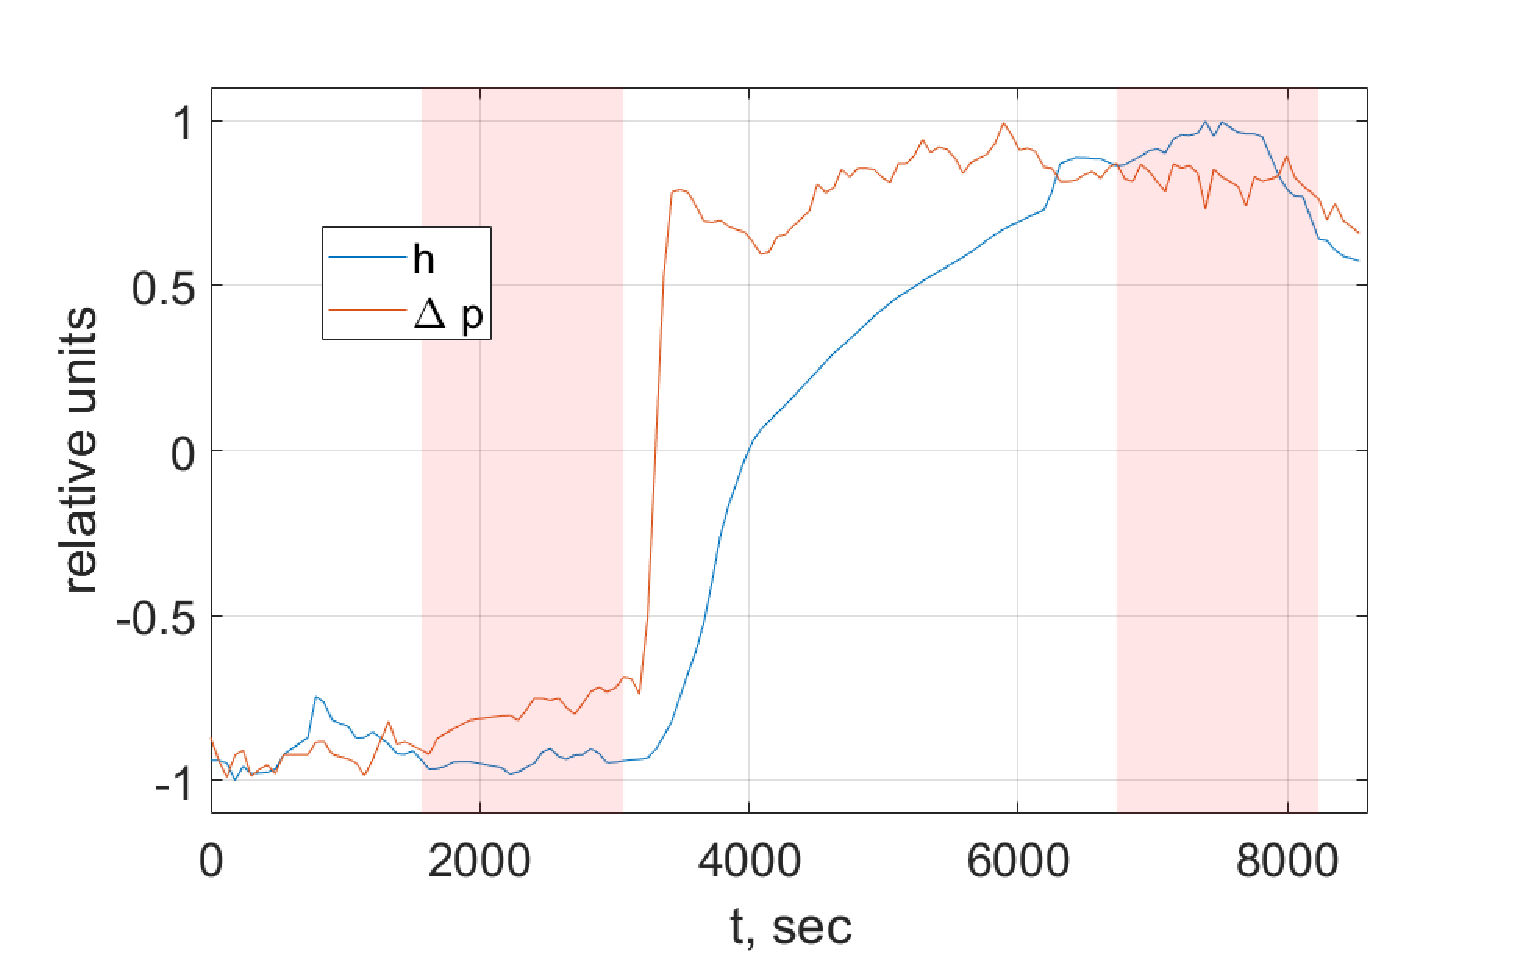
\includegraphics[width=0.48\textwidth]{figs/bad_corr.eps}
    \caption{The detector altitude by GPS module and reconstructed with pressure sensor data. Flight 4-2013, the elevation phase.}
    \label{fig:dp-h-bad}
\end{figure}


\subsection{PMT currents and Background light}

Background light effects the PMT current. Current of the central PMT is shown on the Fig.~\ref{fig:current}. And the night sky background light flux can be evaluated.

.. Dima will write this subsection ...
.. Dima will write this subsection ...
.. Dima will write this subsection ..... Dima will write this subsection ..... Dima will write this subsection ..... Dima will write this subsection ..... Dima will write this subsection ..... Dima will write this subsection ..... Dima will write this subsection ..... Dima will write this subsection ..... Dima will write this subsection ..... Dima will write this subsection ..... Dima will write this subsection ..... Dima will write this subsection ...


\subsection{Pulse noise}

{\Russian

В русле дальнейшего сравнения моделирования для СФЕРЫ с экспериментальными данными был проверен шум импульсный, наблюдающийся невооружённым глазом в отдельных каналах.

Первое, были вычислены коэффициенты корреляции между отдельными каналами. Брались данные 2013 года, все события от ШАЛ и линии, а также их калибровочные кадры. Данные проверялись на синхронность всех каналов (случаются выбросы). В кадрах с отступом в 10 бин от края кадра брались 300 бин до триггера и 300 бин до синхроимпульса в событиях и в линиях, и только первые 300 бин в калибровочных кадрах. Полученные коэффициенты корреляции приведены на рисунке channel correlation. Видно, что ряд каналов неплохо коррелируют друг на друга, т.е. имеют некий общий вклад поверх независимого шума от светового фона.

На тех же данных были получены ковариации каналов. В предположении, что в каждом канале поверх независимого оптического фона накладывается с какой-то амплитудой общий для всех каналов шум аппаратуры были оценены вклады этого общего аппаратного шума в каждый канал (как величина равная сумме всех коэффициентов ковариации данного канала со всем остальными каналам, нормированная на самую большую такую сумму). Оценка не является точной, но это поправимо. Полученные коэффициенты см в файле channel correlations.txt.

Т.к. предполагалось, что "коррелированный" шум носит импульсный нерегулярный характер, то в каждом событии была выделена скоррелированная шумовая составляющая как сумма всех каналов с учётом полученных чуть выше коэффициентов. Т.к. в каждом временном бине суммировались данные с весами, равными ожидаемому вкладу шума в этот канал. Случайный шум от оптического фона должен давать 0, как сумма 109 независимых случайных величин с мат.ожиданием 0. А вот общий для всех шум, одинаковый во всех каналах, должен сложиться и стать заметным.
Эта процедура была проделана со всеми теми же данными (см. Noise.jpg). Если развернуть поближе (Noise  closeup.jpg), то видно, что шум действительно импульсный и имеет некую повторяющую структуру из выброса вверх (светлая полоса), за ним выброса вниз (тёмная полоса), затем небольшое плато, выброс вниз, затем выброс вверх. чтобы выяснить, так ли это и является ли это общей закономерностью всегда, развёртки отдельных событий были выровнены по шумовым импульсам (Nsync.jpg). Шум в итоге регулярный, имеет постоянную амплитуду во всех событиях (т.е. это наводка на аппаратуре, не на ФЭУ, т.к. тут не применены коэффициенты калибровки).
Сумму всех событий с учётом синхронизации шумовых импульсов см. на noise full length (или выделенный повторяющийся сегмент на noise segment). Шаг повторений 252 бина, что соответствует частоте 317460-317800 Гц (но это уже не ко мне, что там так шумит). В остатке имеем, что во всех кадрах присутствует вот такая наводка on the Fig.~\ref{fig:pulse_noise_segment}  c шагом повторений 252 бина по времени.

}


\begin{figure}[tb]
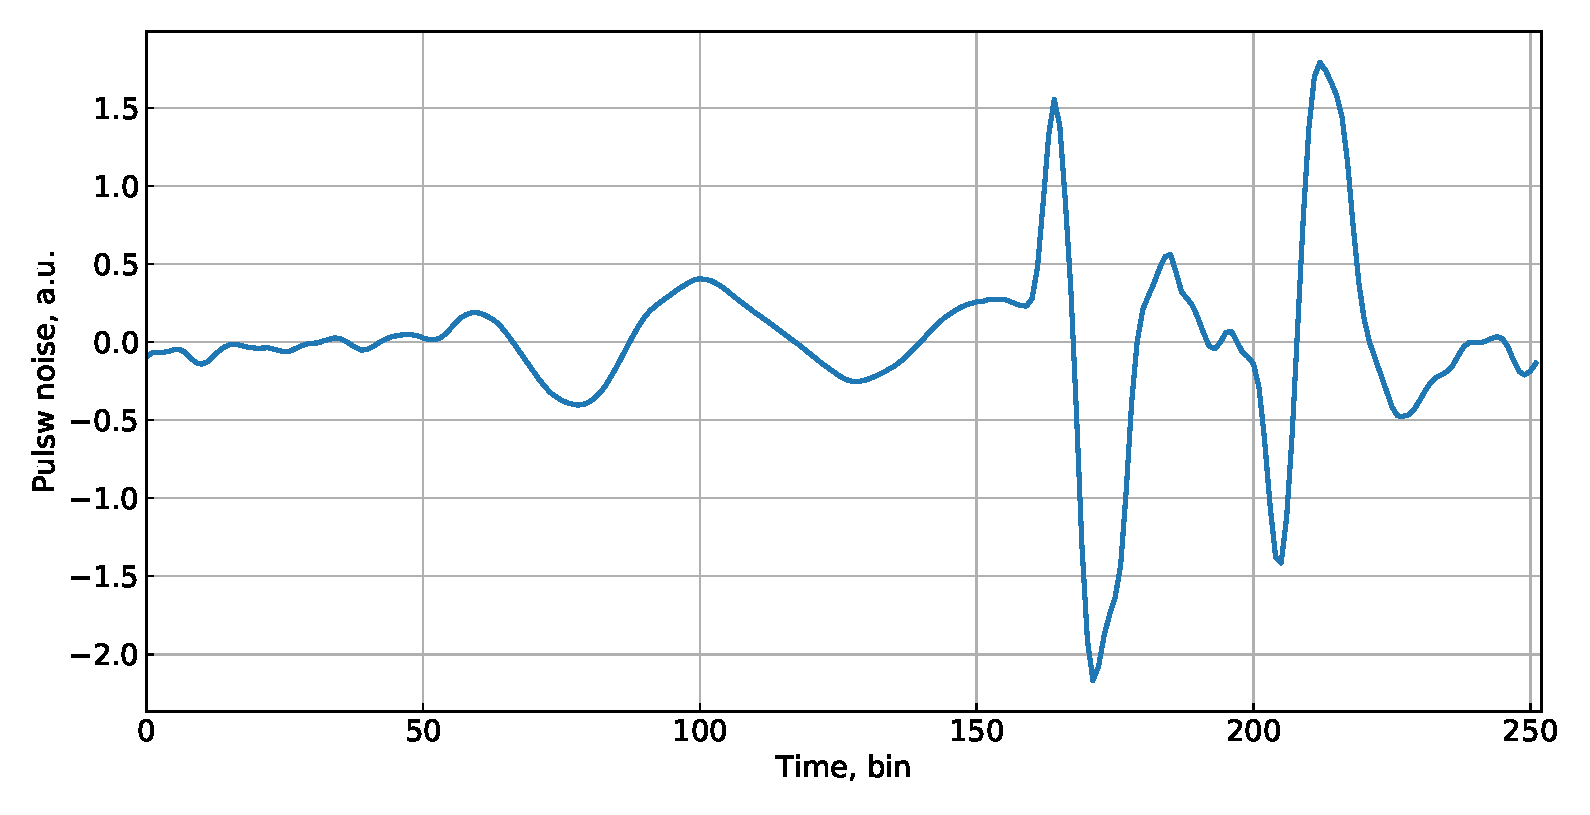
\includegraphics[width=0.48\textwidth]{figs/pulse_noise_segment.eps}
\caption{Pulse noise segment}
\label{fig:pulse_noise_segment}
\end{figure}



\section{Corrections}

The position and inclination of the SPHERE-2 detector are the important values to correct calculations of detected EAS Cherenkov light characteristics. In contrast to ground-based Cherenkov light installations, the detector SPHERE-2 has a variable recording area depending on both the altitude and the inclination angle of the detector.

%%%%%%%%%%%%%%%%%%%%%%%%%%%%%%%%%%%%%%%%%%%%%%%%%%
%\begin{figure}[tb]
%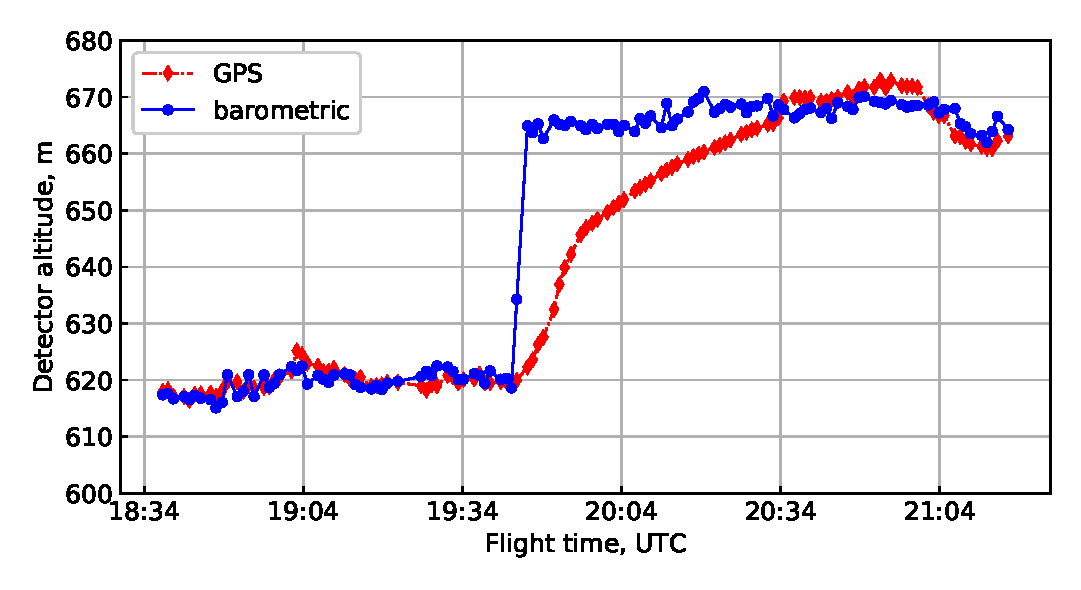
\includegraphics[width=0.48\textwidth]{figs/gps_barometer.eps} 
%\caption{The detector altitude by GPS module and reconstructed with pressure sensor data. Flight 4-2013, the elevation phase.}
%\label{fig:h_gps-hpa}
%\end{figure}

\begin{figure*}[bth]
\centering
%\includegraphics[width=0.44\textwidth, bb= 100 100 900 900,clip]{figs/fov.eps}\hspace{2pc}%
\includegraphics[width=0.9\textwidth]{figs/fov.eps}
%\vspace{10pt}
%\includegraphics[width=0.49\textwidth]{figs/fov_log.eps}%
\caption{The PMTs' fields of view for detector at altitude $H=$ 1000~m. There are presented calculated FOV of PMTs 1, 5, 14, 29, 50 and 77 as indicated on the Fig.~\ref{fig:retina} in assuption of vertical detector optical axis position. The inclinations of the PMTs axis from the SPHERE detector optical axis change from 0 to 26 degrees uniformely.}
\label{fig:pmt_fov}
\end{figure*}


%%%%%%%%%%%%%%%%%%%%%%%%%%%%%%%%%%%%%%%%%%%%%%%%%%%

\subsection{GPS altitude correction by the barometer data}

The observation area depents on the detector altitude $H$ as a square function. To provide the altitude values GPS module, onboard barometer and barometer at the starting point on the Baikal ice surface level with minute-by-minute measurements are used. One can expect GPS height $h$ and difference between surface level and ballon level pressures $\Delta p = (p_{surf} - p_{air})$ to behave consistently because of pressure dependance on height. Other major parameters that affect pressure, such as temperature and humidity, affect both $p_{surf}$ and $p_{air}$ and their effects at least partially cancel each other out in $\Delta p$.

This expected consistent behavior is observed when balloon altitude is generally stable. On Fig. \ref{fig:dp-h-good} such region is shown in the flight 3 data. $h$ and $\Delta p$ are normalized and filtered with high-pass digital Butterworth filter with cutoff frequency $0.83$ mHz ($T=20$ min). It's clear that short-term fluctuations of GPS height and pressure difference are in good correlation. Correlation coefficient is $0.96$ for this data and not less than $0.9$ for all other flights' stable altitude regions filtered the same way. From this we conclude that GPS data are reliable when altitude is relatively stable and surface-air pressure difference directly indicates rapid fluctuations in height.

However, there are regions in data in which $h$ and $\Delta p$ behave rather inconsistently. On Fig.~\ref{fig:dp-h-bad} such region in the flight 4 data is shown (these data are scaled without any filtering). When barometer data change rapidly indicating sudden lift of balloon GPS data starts to change with significant delay and in unnatural smoothed fashion. Such regions in GPS data are observed during almost every abrupt changes in balloon altitude. We believe that this is due to some internal algorithm of the GPS module. Module was designed to be used on ships so it probably handles rapid change in height as an error and tries to smooth it.

Internal algorithm of the GPS module is not available so we've made an attempt to reconstruct correct height data based on pressure measurements which are found to be directly linked to height. After we manually identified smoothed regions such as that shown on Fig.~\ref{fig:dp-h-bad} we picked two adjacent regions of relatively stable altitude before and after it (example of these regions is shown on Fig.~\ref{fig:dp-h-bad} with red bands). In these regions pressure and GPS height data behave consistently (in terms of filtered short-term fluctuations) so we assumed that both measurements are valid. Between these regions the GPS height data are invalid and to be replaced with 'barometric' height logarithmic interpolation in the form of $h-h_0 = - a \, \ln(p/p_0)$. Obtained coefficient $a$ describes local atmosphere and is close to widely adopted value of $8$~km.

After the corrections to GPS height data had been made we estimated the atmosphere density profile. The description is in~\ref{sect:atmosphere-profile}.


%%% Data frames
\begin{figure*}[btp]
    \centering
    %\includegraphics[width=\textwidth]{figs/frames.eps}%
    %ebb -v figs/frames_col.pdf -- to know boundaries bb
    \includegraphics[width=0.92\textwidth, bb=0 0 776 386]{figs/frames_bw.pdf}
    \caption{Frames recorded by the SPHERE-2 detector. The baselines are subtracted, time drift is not corrected, calibration coefficients are not applied. a - is an `event' frame, b - calibration frame, c - direct light, d - random noise, e - longtime events}
    \label{fig:frames}
%\end{figure*}

%%% Data frame Pulses and Sums
%\begin{figure*}[btp]
%\centering
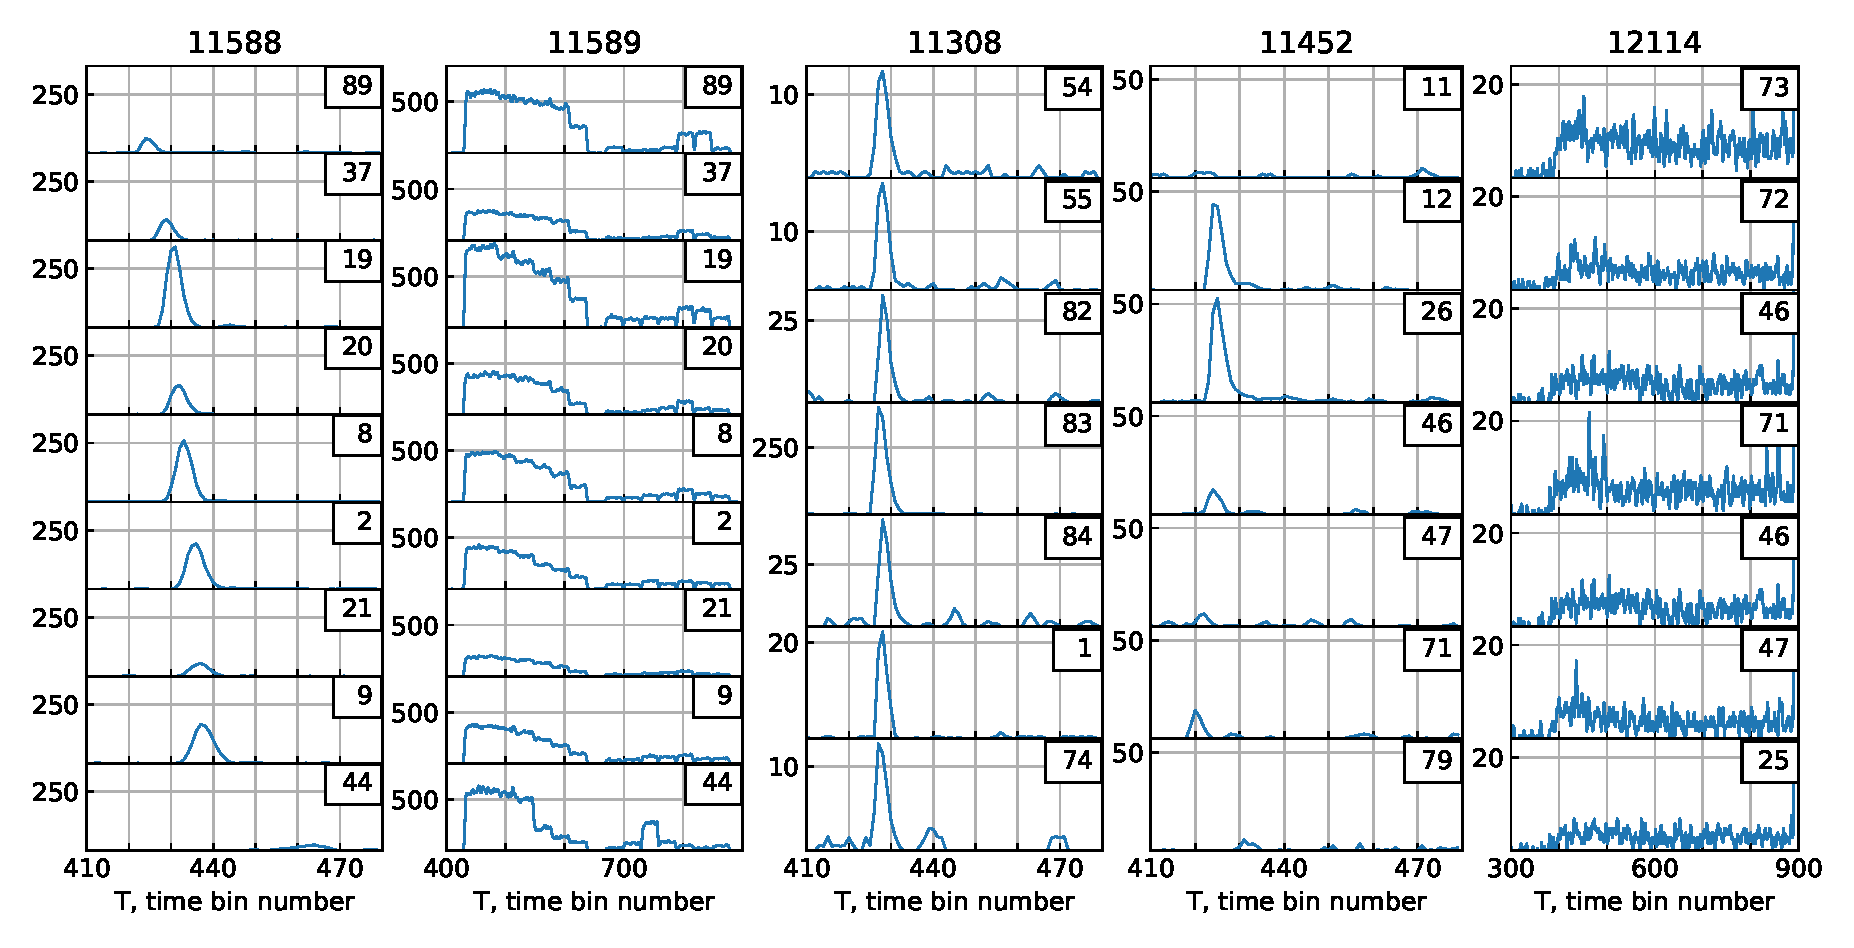
\includegraphics[width=0.9\textwidth]{figs/pulses.eps}%
%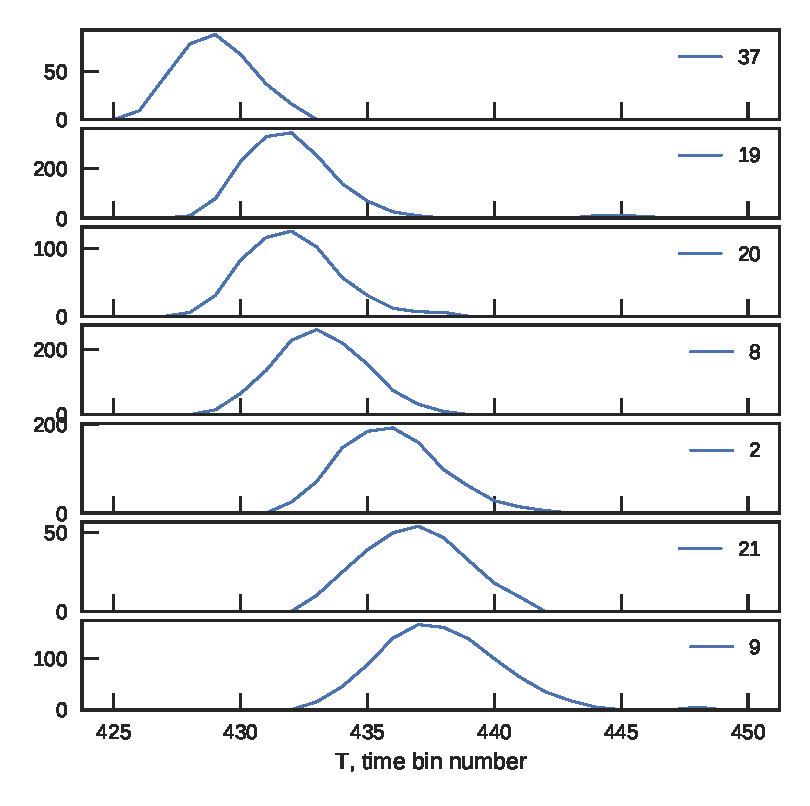
\includegraphics[width=0.5\textwidth]{figs/event_channels.eps}%
\caption{Pulses in channels with maximal signal in the same frames as on Fig.~\ref{fig:frames}. The baselines are subtracted, time drift is corrected, calibration coefficients are applied.}
\label{fig:pulses}
\vspace{1.2pc}
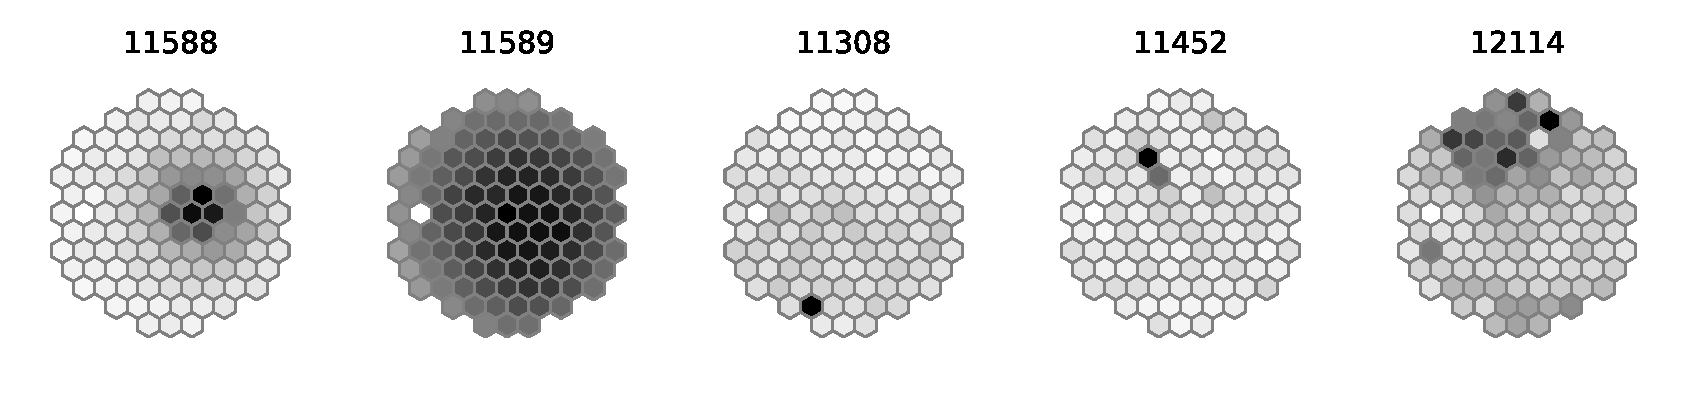
\includegraphics[width=0.9\textwidth]{figs/mosaic_sums_lin.eps}%
\vspace{-1.0pc}
\caption{The sum signal for the events on Fig.~\ref{fig:frames} integrated in time limits indicated on the Fig.~\ref{fig:pulses} x-axis. PMTs are arranged according to the scheme on the Fig.~\ref{fig:retina}. Color intensity of points is proportional to the logariphm of the PMT signal sum.}
\label{fig:mosaic_sum}
\end{figure*}



\subsection{PMTs' field-of-views correction}

In flight during measurements whenever the detector become inclined, the configuration of it's field-of-view (FOV) changed. The FOV of some PMTs shrunk and got closer to the central PMT FOV, for others got larger and moved further from the central PMT FOV. This distorted the reconstructed Cherenkov LDF in spatial terms. Also, change in FOV orientation meant change in optical distance from which the PMT collects light (which affected time measurements). Another issue was the relevant change in average angle under which the snow surface was observed by PMT, which changed light scattering effectiveness (and this distorted the LDF in terms of signals values). In other words, the mosaic inclination if compared to the ground based experiments resulted in measuring stations repositioning with grid distortion and in gradual change in stations sensitivity.

In addition to the full Monte Carlo simulation of the SPHERE detector described in~\cite{ant19} the calculations of detector's optics and PMTs' FOV was performed. The detectors optical scheme is presented on the Fig.~\ref{fig:optics}. The detector was set at 1000~m altitude with zero inclination above flat horizontal observation level. The ground level was divided by the square mesh $[X;Y]$ with 1~m step. From each ground square the weighted photons were emitted towards the detectors diaphragm. The diaphragm was divided into $[x;y]$ mesh with 5~mm step. From each ground square a total of 25600 photons were emitted towards the detector. Each photon weighted by the snow reflectivity coefficient $k_{snow}$ (taken as 0.95~\cite{war82}), by the $\cos^2(\theta)/2$ to account for Lambertian scattering (the $\theta$ is the angle between the direction to the detector and Z-axis), by the distance factor $2\pi{}S/(H^2+(X-x)^2+(Y-y)^2)$ and additional $\cos\theta$ to account the non-normal ray incidence on the diaphragm {\color{red}plus} the normalization coefficient of 2.

At the detector diaphragm level the photons were checked whether they passed the the diaphragm successfully or not and were traced further. At the mosaic level (the mosaic geometrically is a domed {\color{red}tflightcated} cone) the photons were checked that they missed back side of the mosaic and were traced further to the mirror. At the mirror the photons were reflected and additionally weighted by the mirror reflectivity coefficient $k_{mirr}$. During different seasons of observations this coefficient changed as the mirror degraded, so for data analysis the coefficients were selected accordingly to {\color{red} measured ones}, $k_{mirr}$ was about 0.75--0.80 during 2011--2012 seasons and $k_{mirr}$=0.95 for the new mirrors in 2013. After the photons were reflected by the mirror, they were traced back to the mosaic level and check for successfully hitting it. At this step the photons were checked whether they hit any PMT or mosaics blind material. The \mbox{FEU-84-3} PMT's photocathode has 26~mm diameter sensitive area. The spacing between photocathode centers in out mosaic was 44.5~mm, so only 30\% of the mosaic was sensitive to the light. For each photon at the PMT glass surface the glass mirroring coefficient $k_{PMT}$ was calculated, the photon's polarization was selected randomly.

Tracing photons from the full ground grid allowed to find each PMT's FOV and to determine the light collection efficiency for each point on the ground (e.g. how many of the photons that reach the snow surface will be collected by the detector).
Fig.~\ref{fig:pmt_fov} shows the field of view of PMTs with different deviation angles  from the detector optical axis in an assumption of vertical detector optical axis position. There are presented calculated FOV for PMTs with numbers 1, 5, 14, 29, 50, 77 as they are indicated on the Fig.~\ref{fig:retina}. The declination angles of presented PMTs change from 0 to 26 degrees in dependence of the PMT's distance from PMT retina center on Fig.~\ref{fig:retina}. The PMT1 is the Hamamatsu photodetector that has the larger sensitive photocathode area than others FEU-84-3 PMTs, it is seen clearly on the Fig.~\ref{fig:pmt_fov}. 

The same calculations was made for the detector position with different detector axis inclination angles. From the known PMT FOV the coordinates for FOV center were obtained and later used in shower arrival direction reconstruction and shower axis location.


%%%%%%%%%%%%%%%%%%%%%%%%%%%%%%%%%%%%%%%%%%%%%%%%%%%%%%%%%%%%%%%%%%
%%%%%%%%%%%%%%%%%%%%%%%%%%%%%%%%%%%%%%%%%%%%%%%%%%%%%%%%%%%%%%%%%%
\section{Event selection\label{sect:classification}}

\subsection{Trigger data}

The SPHERE-2 detector registered more than 30 thousands trigger event frames but not all of them was caused by signals of the EAS Cherenkov light. 
Examples of `event' frames detected by the SPHERE-2 detector are presented on the Figs.~\ref{fig:frames}, \ref{fig:pulses} and \ref{fig:mosaic_sum}. They are of different types of  dataframes. 

The Fig.~\ref{fig:frames} present events as a full map of signal intensities in all PMT channels during the frame time. The x-axis on the Fig.~\ref{fig:frames} is the detector PMT number $N$ according to Fig.~\ref{fig:retina} and the y-axis is the 12.5~ns time bin number $T$. The color intensity of every point on the Fig.~\ref{fig:frames} is proportional to the logarithm of the signal of the  photomultiplier $N$ in the time bin $T$. Few measuring channels sometimes failed or worked incorrectly. The data of such channels were not processed and are visible in the figures as zeros.

Fig.~\ref{fig:pulses} shows signal pulses in channels with the largest signal magnitudes in the event frame. And the Fig.~\ref{fig:mosaic_sum} demostrates an integral signal for every optic channel. The integration was made as a sum of signals in time limits indicated on the Fig.~\ref{fig:pulses} for every frame respectively. 


\begin{figure}[bt]
    \centering
    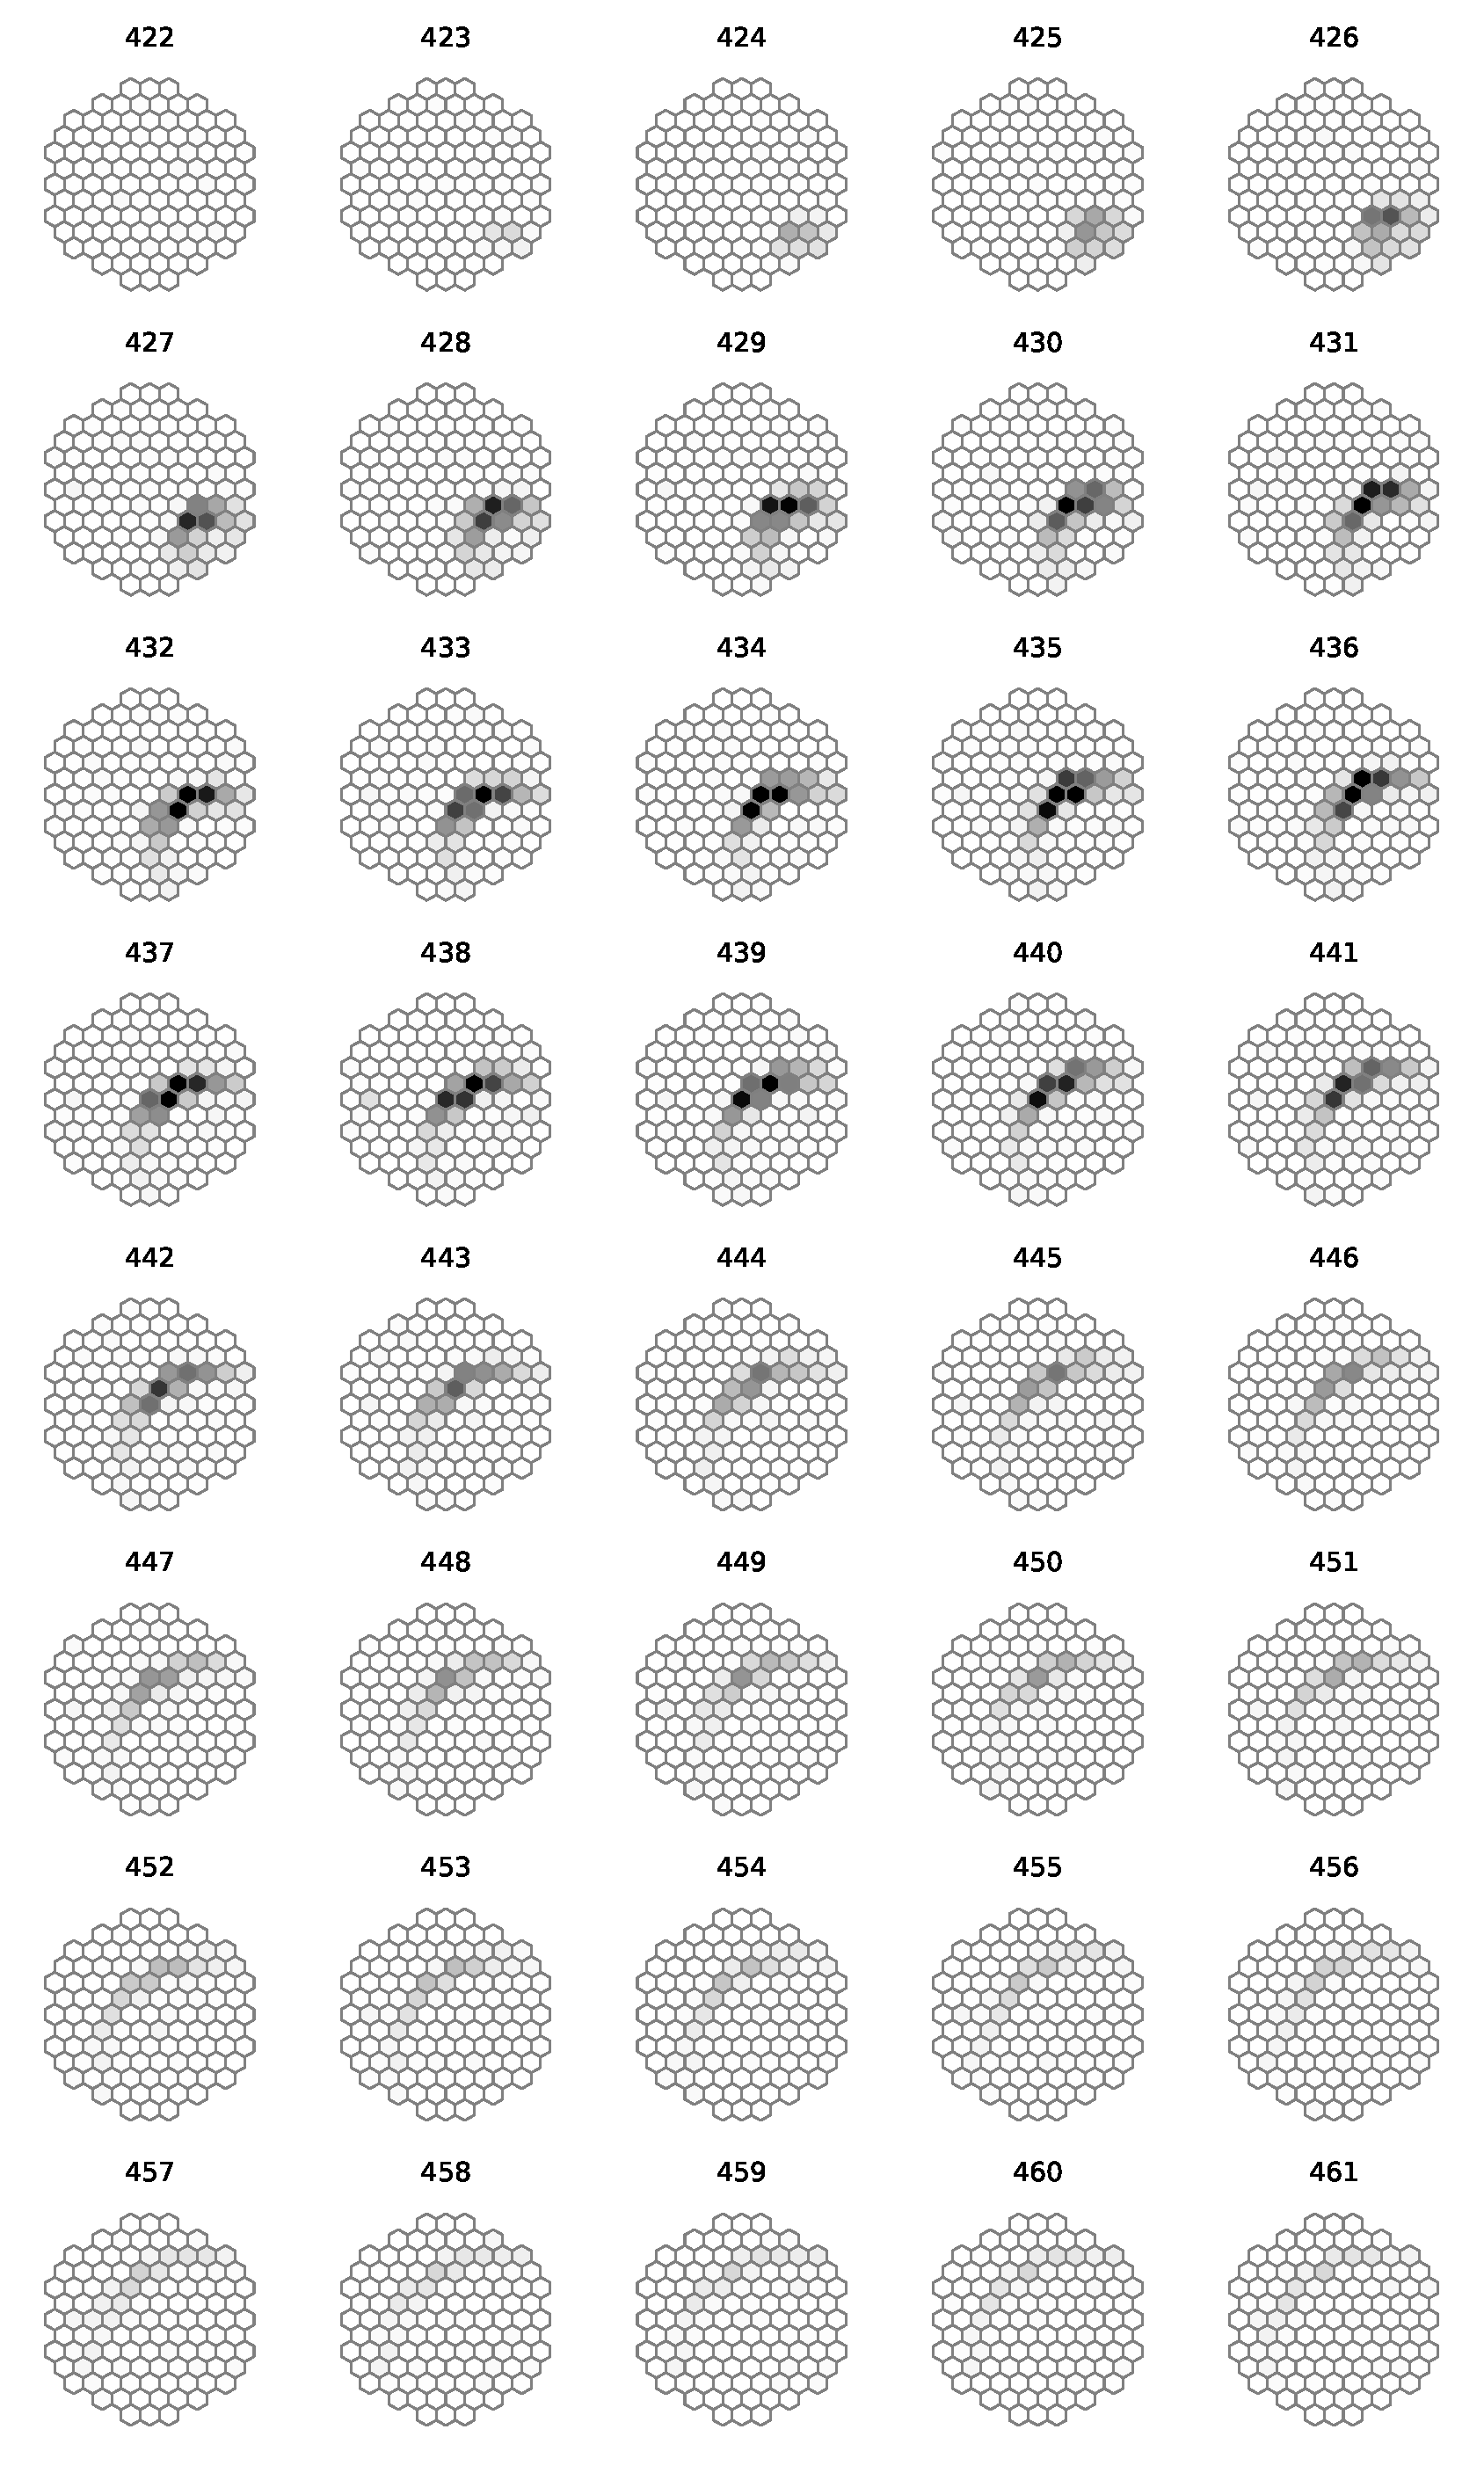
\includegraphics[width=0.48\textwidth]{figs/retina_11588_lin.eps}%
    \caption{The signals of the PMT retina with time step 12.5~ns for the EAS classified event with number 11588 the same as on Fig.~\ref{fig:frames}a, Fig.~\ref{fig:pulses}a, Fig.~\ref{fig:mosaic_sum}a. Zenith angle of the EAS initial particle is estimated as $\theta = 23^{\circ}$.}
    \label{fig:retina_eas}
\end{figure}


\subsection{Trigger event zoo}

The `event' frame 11588 on the Fig.~\ref{fig:frames}a, \ref{fig:pulses}a and \ref{fig:mosaic_sum}a is an EAS-caused event, it is an image of reflected from the snow surface EAS Cherenkov light. The event structure is typical for Cherenkov light frames as it was described in our paper dedicated to simulation of the SPHERE-2 detector experiment~\cite{ant19}. The event was detected from altitude 702~m above show surface. The inclination of the detector was $1.5^{\circ}$

On the Fig.~\ref{fig:retina_eas} this event is represented step by step as a sequience of images with 12.5~ns interval. It is clearly seen how the signal of reflected from the snow Cherenkov light goes through the PMT retina.

The frame 11589 on the Fig.~\ref{fig:frames}b, \ref{fig:pulses}b and \ref{fig:mosaic_sum}b is the `calibration' event following the event 11588. It has the special time signal structure and big magnitudes in all channels caused by LEDs flushes. Calibration frames are separated to calculate the every measuring channel calibration coefficients as desctibed in~\cite{ant16}.

Event 11308 on Fig.~\ref{fig:frames}c, \ref{fig:pulses}c and \ref{fig:mosaic_sum}c is an event caused by simultaneous short pulses in the several photomultipliers. Duration of pulses does not exceed 6~time bins or 75~ns. The data frame has a large pulse signal in one PMT almost ten times brighter than the others. This type of events can be caused by a charged particle passed through the glass or dinode system of photomultipliers or by a local PMT discharge flash.  

Events like 11452 on Fig.~\ref{fig:frames}d, \ref{fig:pulses}d and \ref{fig:mosaic_sum}d are highly likely random noise events. They has no time structure and was caused by random fluctuations in the environment light or by a very-very weak EAS event. 

A mysterious event type like 12114 is presented on Fig.~\ref{fig:frames}e, \ref{fig:pulses}e and \ref{fig:mosaic_sum}e. The event frame has long pulses in numerous channels. The duration of pulses is more than 6 ${\mu}s$ and exceed the frame time capacity.  This `event' may be triggered by crosstalks of PMTs. Or by some long-time events on the surface or in the atmosphere above the detector. The authors favorite version is that these events are caused by light flashes from the electrical discharges accompanying the Baikal lake ice cracking.


\subsection{Rejection}

All the dataframes are pre-processed, including baselines estimation and substraction, time drift detection and correction as described in~\ref{sect:preprocessing} and the PMT calibration~\cite{ant16}. Then the  selection of the data frames caused by reflected EAS Cherenkov light from all the data amount is performed. Firstly the evident non-EAS events are rejected. In the second stage the special pattern analysis procedure is used to find in event frames Cherenkov light signals. The Table~\ref{tab:rejection} shows event number after every step of the rejection. 

\begin{table}[bth]
    \centering
    \caption{Event selection}
    \label{tab:rejection}
    \vspace{1pc}
    \begin{tabular}{|l||r|r|}
    \hline
    Criteria & Frames rejected & Frames remaining\\ 
    %         & by the criteria & after criteria\\ 
    \hline \hline
    Total         &      & 3813\\
    \hline
    Calibration   & 1901 & 1912\\
    Trig $>$ 220  &  125 & 1787\\
    Trig $<$ 300  &    5 & 1782\\
    Dt   $<$ 200  &    7 & 1775\\
    Dt   $>$  5   & 1200 &  575\\
    Dt   $>$  6   & 1284 &  491\\
    Pattern analysis& 36 &  455\\
    \hline
    \end{tabular}
\end{table}

Calibration frames have not special tags and are separated by the large signal sum and the large pulse duration. The detector was configured to make calibration frame after every trigger event frame. But sometimes during experiment the counting rate of the detector exceeded reception capacity of the detector buffer and it caused the buffer overflow and a failure in its operation so the calibration frame was not recorded. Therefore not exact half of recorded events are calibration ones.
From all 3813 frames recordered in 2013 run near the half of them (1901) was calibration ones. 

The failure of the buffer is seen also as a trigger bit location outside of [220, 300] time interval in the dataframe. So frames with trigger time bin less than 220 and more than 300 time bin was deleted from further consideration. There was 130 frames with this trigger failure.

From the further consideration was rejected frames with small time diration like event 11308 on the Fig.~\ref{fig:frames}c. Due to the experiment geometry the signal from the Cherenkov light cannot has duration less than 6~time bins or 75~ns. This condition cuts 1200 (or 1284) frames. 
The rest number of event was iqual to 491 (or 575 in case of criteria Dt $>$ 5). But not all this events was EAS-caused ones. To separate EAS-caused frames the search for the Cherenkov light flashes were performed with special pattern analysis procedure. % and some methods of ML were used. 


\subsection{Search for the Cherenkov light flashes with pattern analysis procedure}

The \mbox{SPHERE-2} detector features quasi-continuous field of view and viewing fields of neighboring PMTs partially overlapped. This means that the light signal from physical shower cannot end in one channel before it will begin in a neighboring channel. Thus the 3D structure of the shower can be reconstructed using the channel data records and taking time as the Z-axis and the PMTs positions as XY-coordinates. The physical shower light in such data representation will look like an inclined disk.

For the shower search procedure the data in each channel of the `event' frame was filtered from the noise values since the procedure is sensitive to the noise. Data in each channel was smoothed using values from 2 previous time bins (with weights 1/4 and 1/16) and 2 consecutive time bins (same weights) of this channel and data of the same time bin from all 6 neighboring PMTs' channels (with weight 1/6). This procedure removes random noise from the data. After that everything with low amplitude was removed from the data. E.g. in the smoothed record of each data channel all values lower than $1.5\sigma_i$ were replaced with zeroes. After that another pass of the filter removed the isolated data bins, the ones that were shorter than 2 consecutive bins since the physical signal cannot be shorter than this because of the geometrical effects, large field of view of each PMT and Cherenkov pulse shape. 

Next step was data binarization --- each zero value remained zero, every non-zero value was replaced with 1. In this binary array using simple wave algorithm the largest isolated compact spot was identified and stored as a `candidate' spot. If the number of PMT's that this `candidate' spot saturated was larger than 7, then the `candidate' spot was checked that it had correct geometry (positive curvature and no secondary large pulses in any PMT) and promoted to the `EAS event' status.


\begin{figure}[t]
    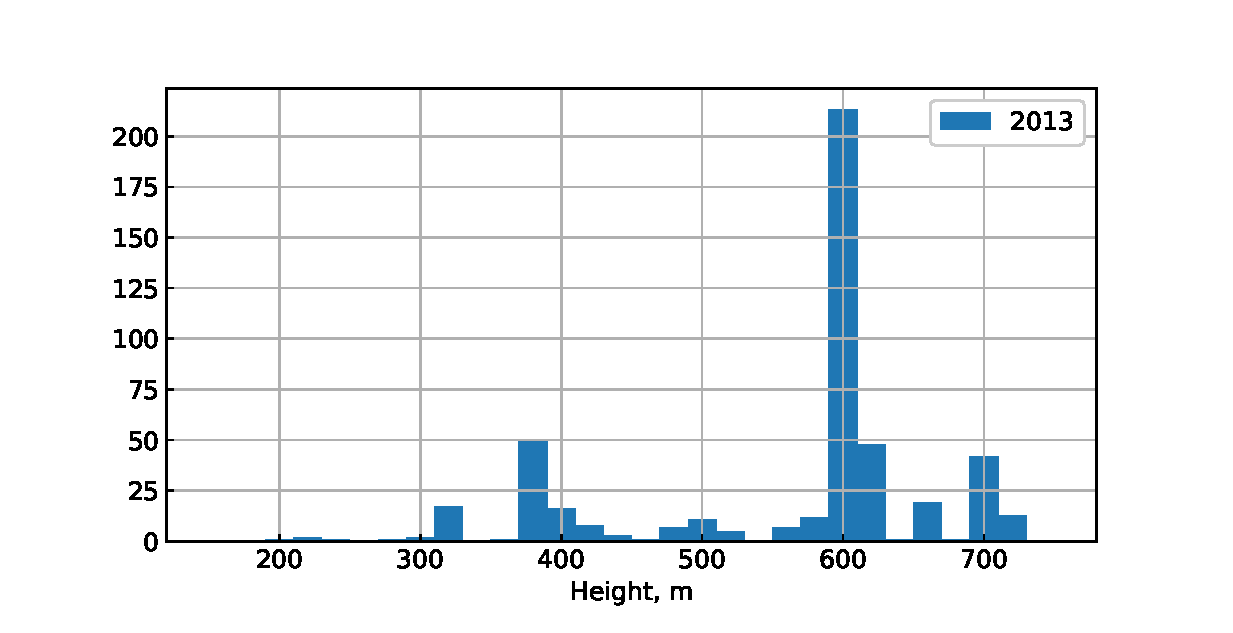
\includegraphics[width=19pc]{figs/height_eas.eps}\hspace{2pc}%
    \caption{The altitude distribution of detected EAS events in 2013.}
    \label{fig:height_eas}
\end{figure}


The altitude distribution of detected events classified as EAS is shown on the Fig.~\ref{fig:height_eas}. The main statistics of 2013 year was collected at altitude near 600~m above ice level. The numbers of triggers classified as EAS events is presented in the Table~\ref{tab:EASstatistics}.


\begin{table}[h]
    \centering
    \caption{The annual statistics of detected EAS.}
    \label{tab:EASstatistics}
    \vspace{1pc}
    \begin{tabular}{|c||c|r|c|r|r|}
    \hline
    run  &  EAS\\ 
    year &  number\\ 
    \hline \hline
    2008 &   1\\  
    2010 &  36\\
    2011 & 220\\
    2012 & 364\\
    2013 & 459\\
    \hline
    \end{tabular}
\end{table}


\section{Conclusions \label{sect:conclusions}}

{
\Russian

В статье мы описали как в эксперименте мы измеряем параметры установки  СФЕРА-2, важные для восстановления черенковских событий.  В частности, высота установки над уровнем земли измеряется двумя способами, что позволяет определить истинное значение высоты. Мы видим, что установка стабильна в воздушном потоке.} 
In the paper we demonstrated how the monitoring of the SPHERE-2 parameters works. 

{
\Russian
Зарегистрированный установкой сигнал очищается от аппаратных эффектов. Мы выявили и учли импульсный шум аппаратуры каналов, влияние звездного фона. 

Зарегистрированные события подверглись классификации. Из них выделены события от черенковского света ШАЛ. }The EAS event selection procedure is described.

{
\Russian
Процедура восстановления параметров ШАЛ будет описана в последующих публикациях.
}


\section*{References}
\bibliography{Sphere-Data.bib}


%%%%%%%%%%%%%%%%%%%%%%%%%%%%%%%%%%%%%%%%%%%%%%%%%%%%%%%%%%%%%%%%%%%%%%%%%
%%%%%%%%%%%%%%%%%%%%%%%%%%%%%%%%%%%%%%%%%%%%%%%%%%%%%%%%%%%%%%%%%%%%%%%%%
%%%%%%%%%%%%   Appendix %%%%%%%%%%%%%%%%%%%%%%%%%%%%%%%%
%%%%%%%%%%%%%%%%%%%%%%%%%%%%%%%%%%%%%%%%%%%%%%%%%%%%%%%%%%%%%%%%%%%%%%%%%
\appendix

\section{Atmosphere density profile\label{sect:atmosphere-profile}}

\begin{figure}[bt]
\centering
\begin{minipage}[t]{0.48\textwidth}
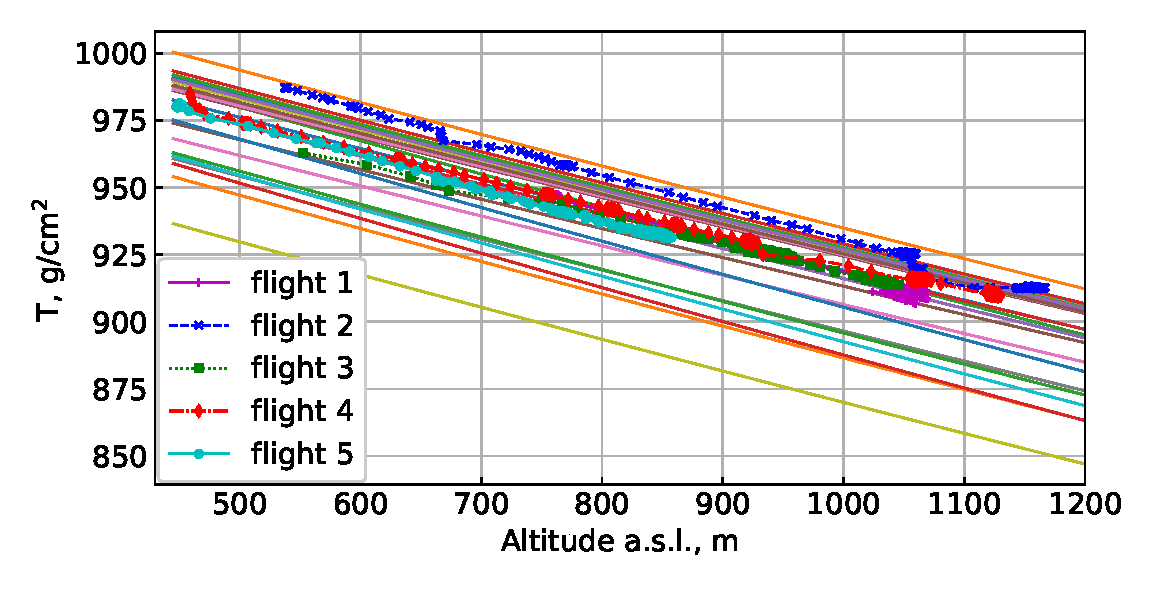
\includegraphics[width=\textwidth]{figs/atmosphere_T.eps}
\vspace{-1.0pc}
\caption{Mass overburden versus height points in each flight and CORSIKA profiles. Solid black line represents profile adopted in the preliminary modelling}
\label{fig:massoverburden}
\end{minipage}
\vfill
\vspace{1pc}
\begin{minipage}[t]{0.48\textwidth}
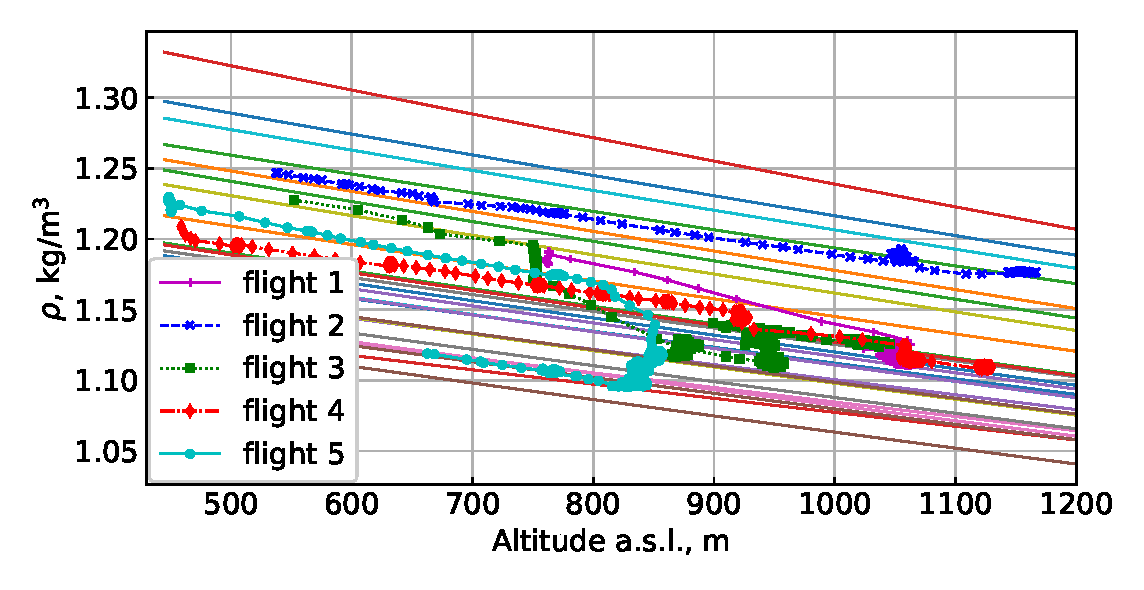
\includegraphics[width=\textwidth]{figs/atmosphere_rho.eps}
\vspace{-1.0pc}
\caption{Density versus height points in each flight and CORSIKA density profiles (negative derivatives of the curves in fig. \ref{fig:massoverburden}). Solid black line represents profile adopted in the preliminary modelling}
\label{fig:density}
\end{minipage}
\end{figure}


After the corrections to GPS height data were made we estimated the atmosphere density profile. Direct measurements with onboard barometer and thermometer were taken at less than 1000~m above the ice therefore information about higher atmosphere is not available. To obtain the best extrapolation of these data we had to use the set of previously measured and parametrised atmospheres provided in CORSIKA software \cite{hec98}.

In CORSIKA atmosphere is described with mass overburden $T(h) \equiv \int_{h}^{+\infty} \rho(x) dx$. The $T(h)$ variation with altitude is modeled by 5 layers with mass overburden following an exponential decrease in the lower four and linaer decrease in the highest one.

%\begin{equation}
%T_i(h) &= a_i + b_i \cdot \exp(-h/c_i), \; i = 1,\dotsc,4 \\
%T_5(h) &= a_5 + b_5 \cdot h / c_5
%\end{equation}

Layer boundaries are selected in a manner that the overall function $T(h)$ can be differentiated continuously. CORSIKA provides 26 atmosphere models corresponding to measurements taken at different seasons in different locations around the globe. For each atmosphere experimantal range of altitudes was fully contained in the lowest layer.

We used following equations to derive mass overburden $T$ and density $\rho$ from measured pressure $p$ and temperature $t$.

\begin{equation}
T     = \frac{p}{g} \\
\rho  = \frac{p \, M}{R \, t} \\
\end{equation}

Here $g$ is the gravitational acceleration, $M$ is the average molar mass of air, $R$ is the gas constant.

Calculated experimental points for $T$ and $\rho$ in each flight are shown in Fig.~\ref{fig:massoverburden} and Fig.~\ref{fig:density}. CORSIKA atmospheres are shown with dashed lines except for the profile that was adopted in the preliminary modelling, wich is shown with solid black line.

It's seen that previously picked atmosphere is inconsistent with experimental data for $T$ in terms of absolute values, but their derivatives lie relatively close. Therefore either full remodelling with better fitting atmosphere or some correction of final data is required to reduce systematic errors in energy and composition estimation.





\section{Data preprocessing\label{sect:preprocessing}}

\begin{figure}[t]
\centering
\begin{minipage}[t]{0.5\textwidth}
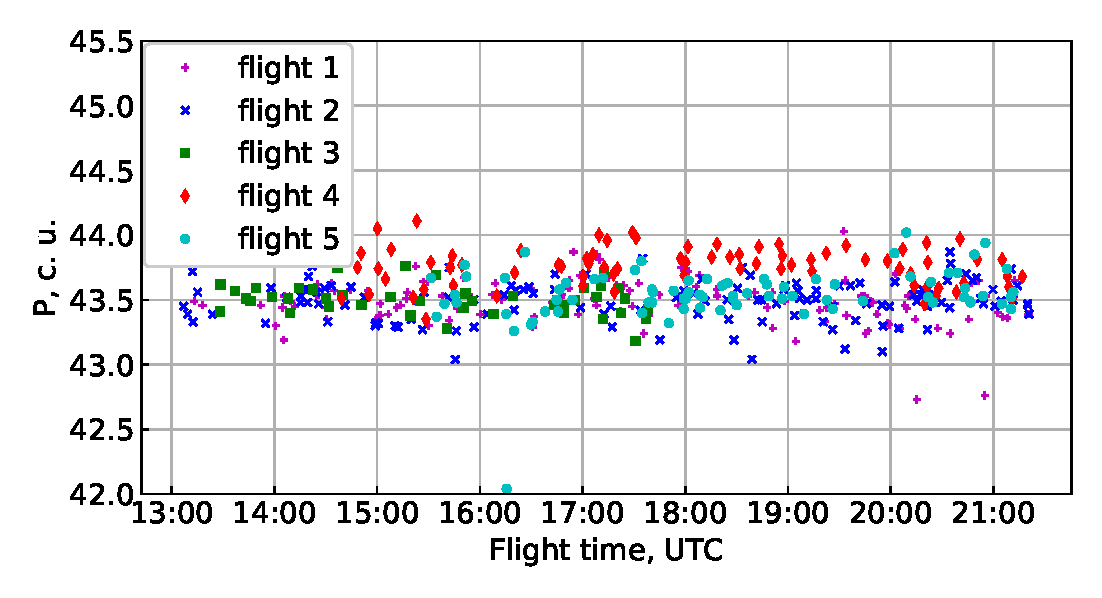
\includegraphics[width=19pc]{figs/pied_PMT1.eps}
\vspace{-1.0pc}
\caption{The PMT baseline for central PMT.}
\label{fig:pied}
\end{minipage}
\vfill
\vspace{1pc}
\begin{minipage}[t]{0.5\textwidth}
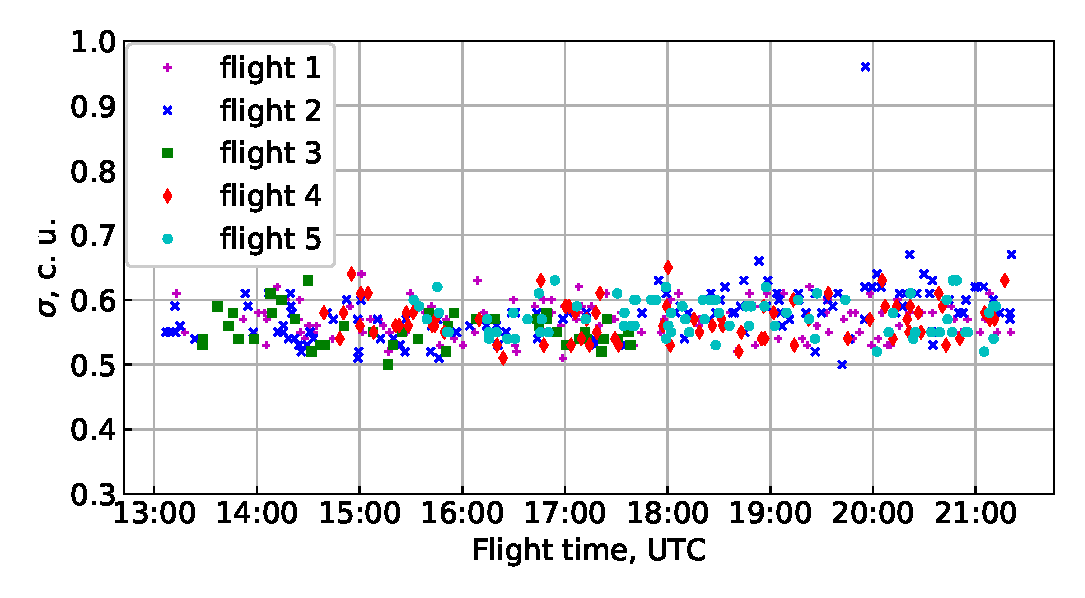
\includegraphics[width=19pc]{figs/piedfluct_PMT1.eps}
\vspace{-1.0pc}
\caption{The PMT baseline fluctuations for central PMT.}
\label{fig:piedfluct}
\end{minipage}
\end{figure}


%\begin{figure}[bht]
%\centering
%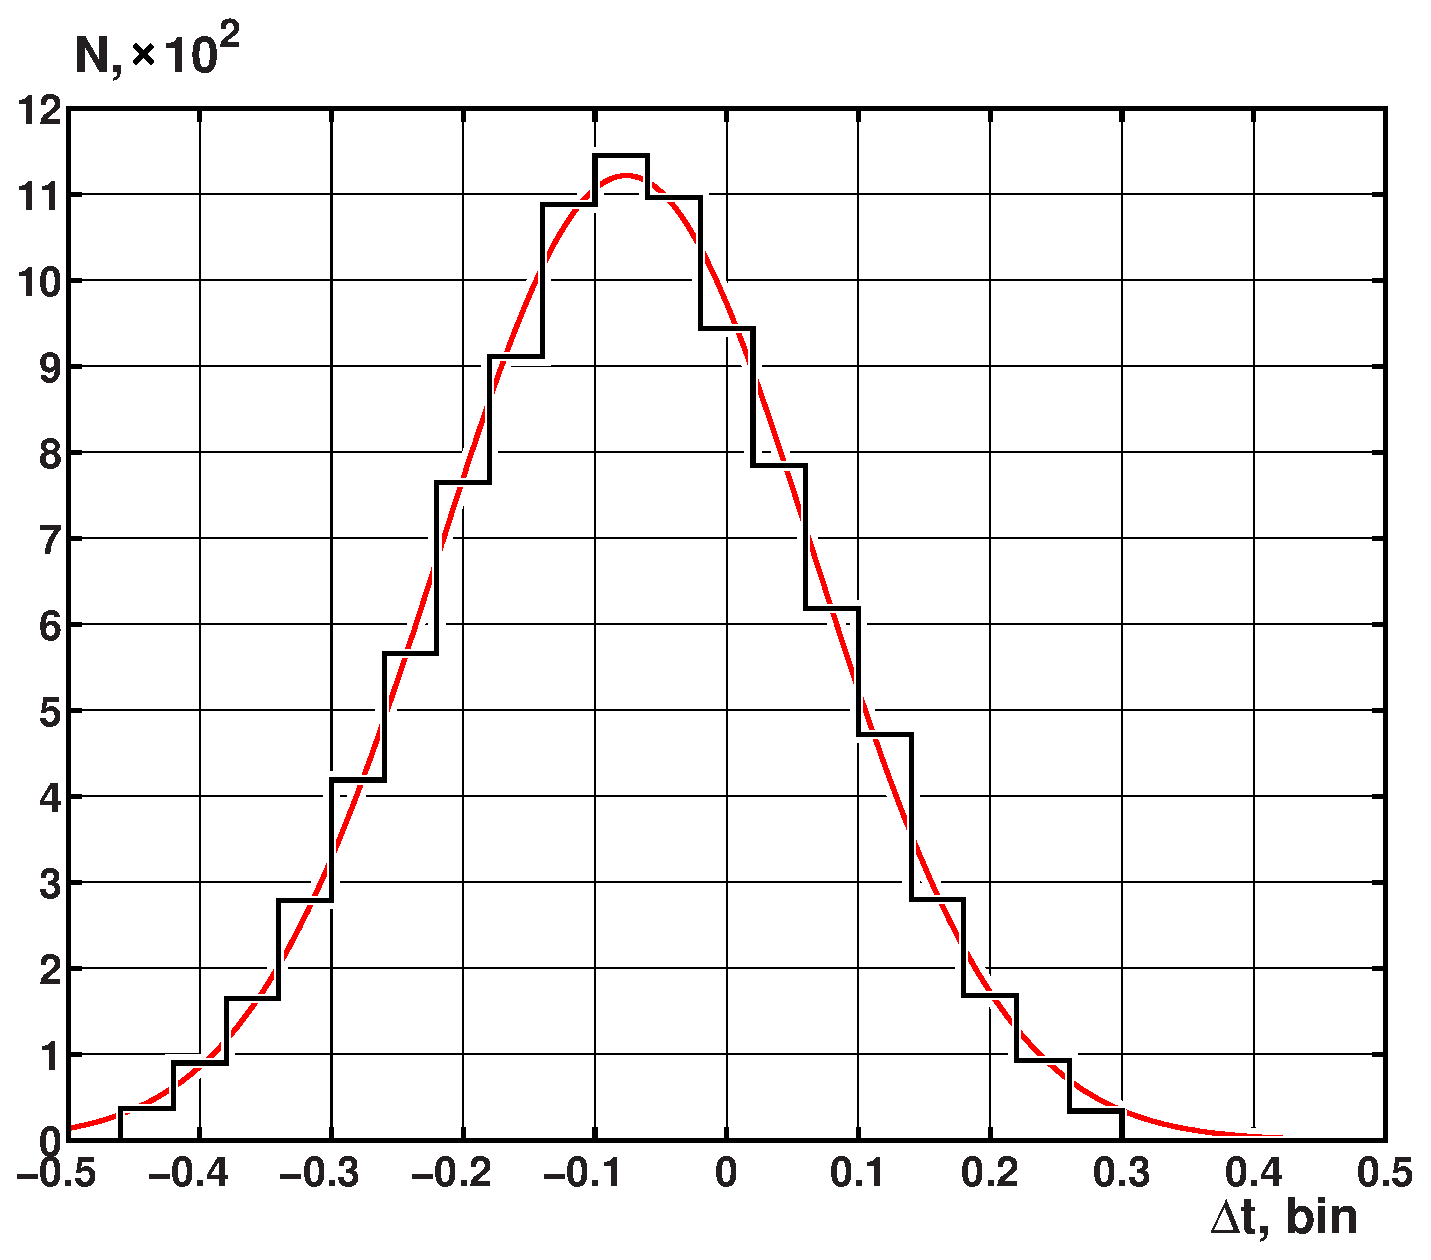
\includegraphics[width=0.40\textwidth]{figs/time_correction_quality_noise_low}
%\caption{The histogram of modeled differences between true and reconstructed synchronization pulse positions.}
%\label{fig:synchro}
%\end{figure} 


\subsection{Baseline handling}

The \mbox{SPHERE-2} DAQ system had two data channels per one PMT working with half phaze shift effectively doubling sampling frequency. Due to some technical reasons (see detailed description of \mbox{SPHERE-2} electronics in \cite{ant15a}) in the DAQ system the current was added to the PMT output before it got to the FADC. This additional baseline current, individual in each channel, resulted in on average about 40--60 additional `code' units (arbitrary unit on the FADC output, see~\cite{ant16} for details) and not necesserilly integer in those units. The exact value of added current was unknown and changed slowly over time with the change of temperature and conditions within the control block (this was observed on-site during days temprature change). The changes of the baseline current were small and slow enough to consider the baseline constant during each recorded frame (during the flight the current changed on about 1--2 units per 4 hours). 

During data preprocessing the baselines in each channel were estimated as an average value from the first 400 time bins recorded, see for example Fig.~\ref{fig:pied}. The better estimation could be achieved by fitting the distribution of all values recorded in the frame (thus rendering procedure less sensitive to extreme fluctuations or random particle signals) with Gaussian distribution function. However during the later signal reconstruction procedure small baseline uncertainties were automatically accounted for, thus simpler and faster procedure was used. After a baseline in a channel was estimated its value was substracted from signals in this channel to have a near-zero signal baseline further. Figs.~\ref{fig:frames}, \ref{fig:pulses} and \ref{fig:mosaic_sum} show events signals with substracted baselines.

Along with average value for each channel the standard deviations of signals in each channel $\sigma_i$ were estimated and found to be from 0.5 to 2.5 arb.\ unit, see  Fig.~\ref{fig:piedfluct}. The fluctuation of the baseline in each data channel came from constant starlight background that was present during the measurements. With the clear moonless night sky starlight background is (1--2)$\cdot10^{12}$~photon~sr$^{-1}$~s$^{-1}$~m$^{-2}$~\cite{starlightbackground}. Thus for 12.5~ns about 50--70 photons from starlight background should had been falling on each PMT on average producing about 4--7 photoelectrons, which translates in 3--5 arb. units. The characteristic amplitude of these fluctuations were individual for each channel and came from differences in amplification and quantum efficiency of each PMT. More sensitive PMTs showed higher fluctuations. The estimated fluctuations are consistent with the expected ones. The electronics and PMTs themselves produced very low noise (less than 1 arb. unit) as was checked in dark room in the laboratory and on-site. The average fluctuation values later were used as thresholds during EAS events identification to filter-out noise. 

\subsection{Channel synchronization}

\begin{figure}[t]
\center
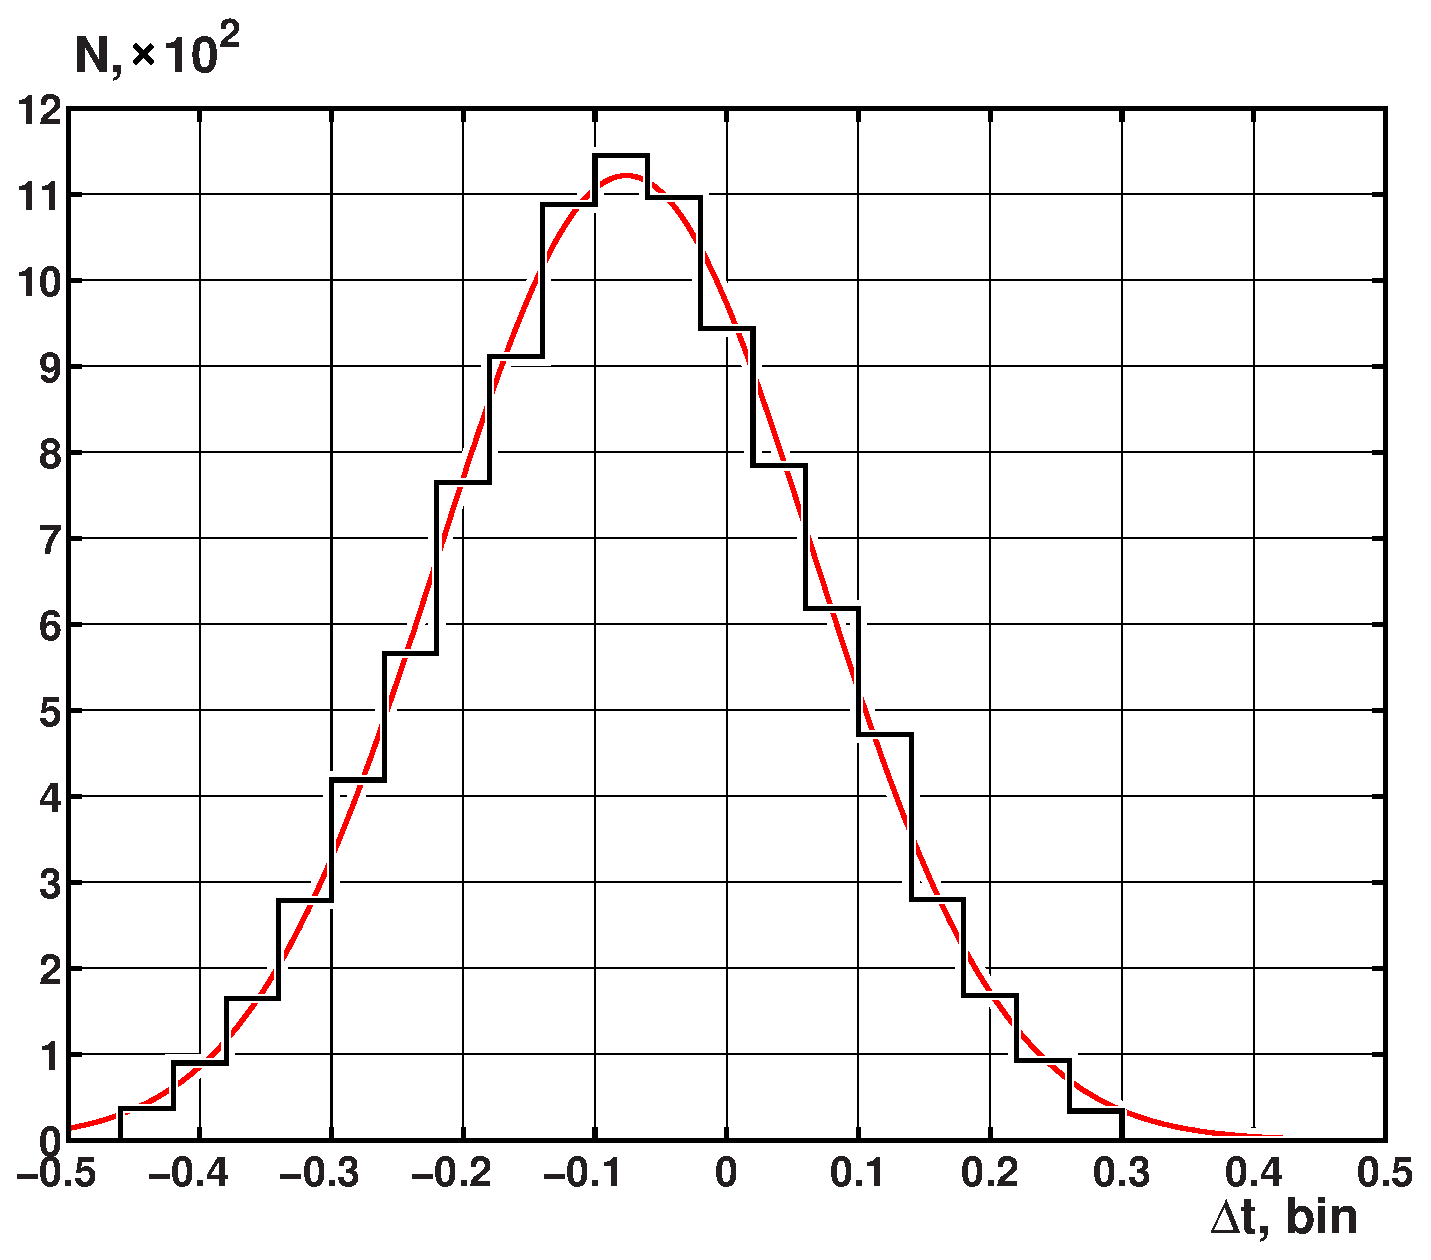
\includegraphics[width=0.35\textwidth]{figs/time_correction_quality_noise_low.eps}
\caption{The histogram of modeled differences between true and reconstructed synchronization pulse positions.}
\label{fig:synchro}
\end{figure} 


Each data recording channel has independent FADC and independent buffer to store data. All FADCs has equal parameters and sampling frequency. So in ideal conditions that would've sufficed to have all channels synchronized via the trigger signal. In real design a flaw was found that sometimes caused the high amplitude signal from PMT to induce the fake `stop-go' signal in buffer control lines thus creating a time drift between channels. In order detect, estimate and compensate this drift the calibration system produced a short all-LED synchronization pulse in 5.8~$\mu$s after the trigger signal. This pulse appeared in the end of the `event' frame and is clearly seen on the Fig.~\ref{fig:frames} at time near bin 900. The calibration LEDs illuminated the PMT mosaic via equal-length optical fibers that were located near the PMT retina. Hence the light pulse falling on the mosaic was physically synchronous in every PMT. 

This pulse with approximate duration of 100~ns was strong (about 400 arb.\ code units) and was easily detectable in each data channel. The center-of-mass approach was uses to find the exact position of the synchronization pulse. The Monte Carlo simulation of synchronization pulse digitalization and automatic center-of-mass estimation was done to determine the procedures precision. 
On the Fig.~\ref{fig:synchro} the results of this simulation are shown. 
The $\Delta{}t$ is the difference between the random initial synchronization pulse position and the reconstructed one. In the best case scenario (high sensitivity PMT) the precision of the pulse location is better that 0.05~time bin, e.g. better than 0.5~ns. In worst case it's more like 2--3~ns. On average the channels synchronization precision was about 1~ns.

In order to simplify `event' frames classification later all channels were shifted (time drift values were rounded to the nearest integer for this purpose) so that the synchronization pulse appeared at predefined time bin. Empty bins at the beginning or the end of the data channel record were padded with zeros. The exact values of time drift after correction (each less than 1 time bin) were stored for later use during shower arrival direction estimation. 

The `calibration' frame (Fig.~\ref{fig:frames}b) paired to each `event' frame did not contain the synchronization pulse. As the `calibration' frame was not used for any kind of time measurements the exact position of calibration pattern in each channel was irrelevant. But for simplification of further procedures all the channel were shifted to put the edge of first all-LED pulse to the predefined time bin.

\end{document}




%%%%%%%%%%%%%%%%%%%%%%%%%%%%%%%%%%%%%%%%%%%%%%%
\begin{figure}[bt]
    \centering
    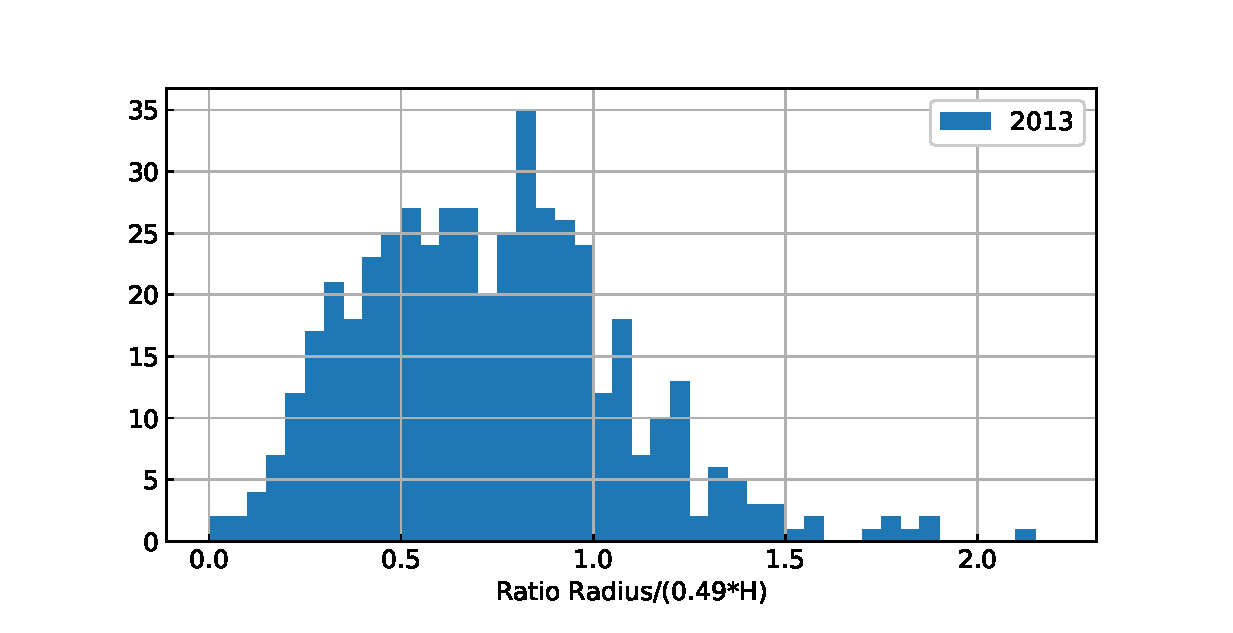
\includegraphics[width=0.48\textwidth]{figs/2013_r_div_H.eps}%
    \caption{The distance of axis from the center of detector FOV. }
    \label{fig:r_div_H}
\end{figure}

 \hfill
    \begin{minipage}[t]{0.47\textwidth}
    \centering
    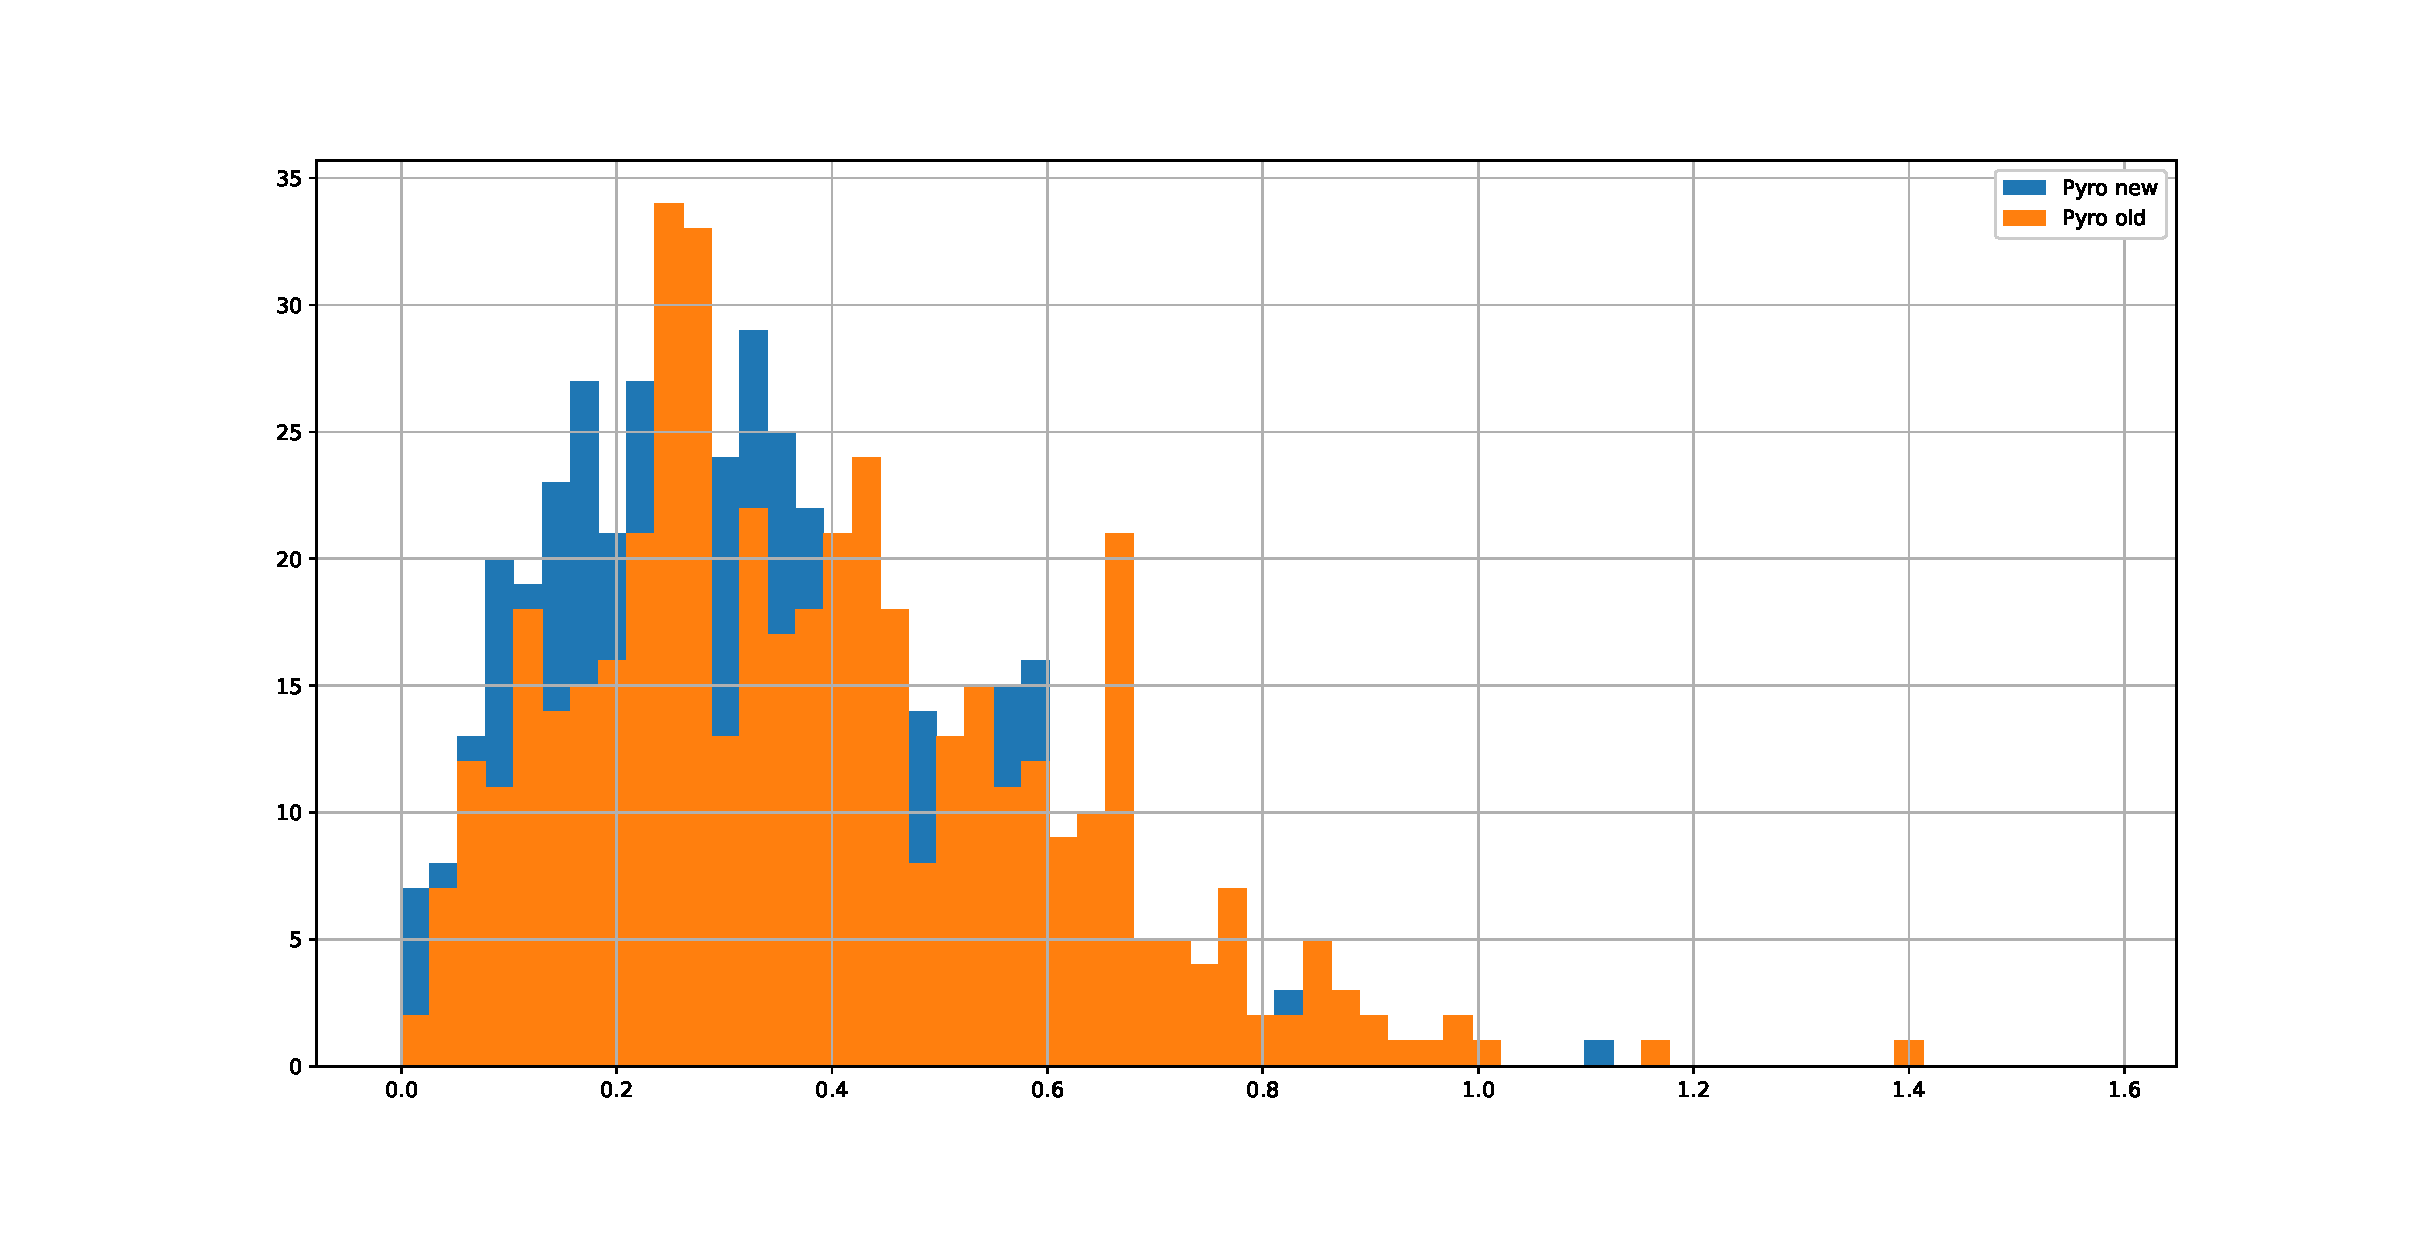
\includegraphics[width=19pc]{figs/theta.eps}%
    %\vspace{-1.0pc}
    \caption{The zenith angle $\theta$ distribution of detected EAS events in 2013.}
    \label{fig:theta_eas}
    \end{minipage}
\end{figure*}

